\documentclass[
    paper=a4,
    fontsize=11pt
]{scrbook}
\usepackage{lecture-notes}  % load custom template
\nocite{*}  % include all reference entries in bibliography

%% PDF INFO %%
\hypersetup{
    pdftitle=Quantitative Foundations of Artificial Intelligence,
    pdfauthor=Marvin Theis{\ss},
    bookmarksopenlevel=1
}

%% BIB-FILE(S) %%
\addbibresource{bibliography/quant-foundations-ai.bib}

%% BEGINNING OF DOCUMENT %%
\begin{document}

%% FRONTMATTER %%
%% TITEL-SEITE %%

% Provide information for title page
\subject{\sffamily Lecture Notes}
\title{Quantitative Foundations\\ of Artificial Intelligence}
\subtitle{Justus-Liebig-Universit\"at Gie{\ss}en \textbar{} Winter 2023/24}
\author{\textbf{Lecturer}: Prof.~Dr.~Ludger Overbeck}  % NOTE: \author is being misused to refer to the lecturer
\date{Last edited on \today}
\publishers{By Marvin Thei{\ss}}

\pagenumbering{Alph}

\begin{titlepage}
    \begin{tikzpicture}[remember picture, overlay]
        \begin{scope}[on background layer]
            % LIGHTBLUE BACKGROUND
            \fill[lightblue] ($(current page.north west) + (8mm, -38mm)$) rectangle ($(current page.south east)$);
        
            % LOGO
            % \node[anchor=north east, inner sep=0pt] (jlu) at ($(current page.north east) - (8mm, 8mm)$) {\includegraphics[width=48mm, height=60mm]{tmp/logo}};
        \end{scope}

        % HEADLINE
        \node[rectangle, anchor=south west, inner sep=0pt, text width=130mm, text=white] (headline) at ($(current page.south west) + (16mm, 32mm)$) {\fontsize{24pt}{34pt}\let\strut\relax\bfseries Quantitative Foundations\\ of Artificial Intelligence \par};

        % SUBHEADLINE
        \node[rectangle, anchor=south west, inner sep=0pt, text width=130mm, text=white] (subheadline) at ($(headline.north west) + (0, 8mm)$) {\fontsize{12pt}{14pt}\bfseries Justus-Liebig-Universit\"at Gie{\ss}en \textbar{} Winter 2023/24 \par};

        \begin{scope}[on background layer]
            % BLUE TEXTBOX
            \fill[blue, fill opacity=0.9] ($(current page.west |- subheadline.north) + (0mm, 16mm)$) rectangle ($(current page.south west) + (154mm, 16mm)$);
        \end{scope}
    \end{tikzpicture}
\end{titlepage}

\cleardoublepage
\pagenumbering{roman}

\uppertitleback{
    This work \copyright{} 2024 by \href{https://github.com/mrvnthss}{Marvin Thei{\ss}} is licensed under \href{http://creativecommons.org/licenses/by-nc-sa/4.0/?ref=chooser-v1}{CC BY-NC-SA 4.0} \ccbyncsa \\

    You are free to distribute, remix, adapt, and build upon the material in any medium or format. You must give \href{https://creativecommons.org/licenses/by-nc-sa/4.0/?ref=chooser-v1\#ref-appropriate-credit}{appropriate credit}, provide a link to the license, and \href{https://creativecommons.org/licenses/by-nc-sa/4.0/?ref=chooser-v1\#ref-indicate-changes}{indicate if changes were made}. You may do so in any reasonable manner, but not in any way that suggests the licensor endorses you or your use. You may not use the material for \href{https://creativecommons.org/licenses/by-nc-sa/4.0/?ref=chooser-v1\#ref-commercial-purposes}{commercial purposes}. If you remix, transform, or build upon the material, you must distribute your contributions under the \href{https://creativecommons.org/licenses/by-nc-sa/4.0/?ref=chooser-v1\#ref-same-license}{same license} as the original.
}

\lowertitleback{
    \textbf{Disclaimer}: This publication is an independent project and is neither affiliated with, nor authorized, sponsored, or approved by Justus-Liebig-Universit{\"a}t Gie{\ss}en. The content within is based solely on my own notes, and should not be taken as an official course material, guide, or representation of the university's views, teachings, or policies. \\

    I have made every effort to ensure the accuracy and completeness of the information contained within, but the document may inadvertently contain errors. I assume no responsibility for errors, omissions, or any inconsistencies herein. \\

    Readers should consider this work as a personal project, intended for general informational and educational purposes only. Any reliance placed on the material in this publication is strictly at your own risk. \\

    \textbf{Feedback and Corrections}: I welcome and appreciate feedback from readers, especially regarding errors or inaccuracies found within this publication. If you notice any mistakes or have suggestions for improvement, please feel free to contact me at \href{mailto:mrvnthss@mail.de}{mrvnthss@mail.de}.
}

\maketitle


%% TABLE OF CONTENTS %%
\tableofcontents
\cleardoublepage

%% MAIN TEXT %%
\pagenumbering{arabic}
%% PART I %%
\part{Statistical Learning Theory}

%% CHAPTER 1 %%
\chapter{Formal Setting}
\label{ch: formal setting}

In this first chapter, we briefly describe the formal setting that will accompany us for the remainder of this course. We will introduce some common machine learning terminology and we will fix some notation.

Throughout this course, we let $(X, Y)$ denote a pair of random variables defined on a common probability space $(\Omega, \mathcal{A}, \P)$, taking values in arbitrary spaces $(\mathcal{X}, \mathcal{F}_{\mathcal{X}})$ and $(\mathcal{Y}, \mathcal{F}_{\mathcal{Y}})$, respectively\footnote{$\mathcal{F}_{\mathcal{X}}$ and $\mathcal{F}_{\mathcal{Y}}$ denote $\sigma$-algebras on $\mathcal{X}$ and $\mathcal{Y}$, respectively. We won't be concerned with measurability in this course, so these won't play an important role.}. Most often, these spaces will be the Euclidean space $\R^d$ of dimension $d$. Also, we may sometimes just write $Z$ for the pair $(X, Y)$. We denote the joint distribution of $X$ and $Y$ by $\P_{(X, Y)}$, i.e.,
\[
    \P_{(X, Y)}(A, B) = \Pr{X \in A, Y \in B}, \quad A \in \mathcal{F}_{\mathcal{X}}, \; B \in \mathcal{F}_{\mathcal{Y}}.
\]
Similarly, we write $\P_X$ and $\P_Y$ for the marginal distributions of $X$ and $Y$, respectively. We will frequently be working with (hypothetical) data in this course. To this end, we let $\mathcal{D}_n = \set{(X_1, Y_1), \dots, (X_n, Y_n)}$ denote a set of $n$ pairs $Z_i = (X_i, Y_i)$, all of which are i.i.d.\ draws from the joint distribution of $(X, Y)$.

%% SECTION 1.1 %%
\section{Conditional Expectation}

To keep things easy, let's assume that we're working in the real numbers $\R$, and let $X$ and $Y$ be two real-valued random variables defined on a common probability space $(\Omega, \mathcal{A}, \P)$ such that $\ex{Y^2} < \infty$. Then, the \emph{conditional expectation} of $Y$ given $X$ is the unique\footnote{This is to be understood in an almost sure sense, i.e., if $Z$ is another random variable satisfying the two properties, then $Z = \Ex{Y \given X}$ almost surely.} random variable $\Ex{Y \given X}$ satisfying
\begin{enumerate}
    \item $\Ex{Y \given X}$ is $\sigma(X)$-measurable,
    
    \item $\int_A \Ex{Y \given X} \, \mathrm{d}\P = \int_A Y \, \mathrm{d}\P$ \quad for all $A \in \sigma(X)$.
\end{enumerate}
Note that, by setting $A = \Omega \in \sigma(X)$, the second property implies $\Ex{\Ex{Y \given X}} = \Ex{Y}$, which is known as the law of total expectation. Moreover, the second property can be rewritten as
\[
    \Ex{\indicator{A} \Ex{Y \given X}} = \Ex{\indicator{A} Y}, \quad A \in \sigma(X),
\]
and this can be generalized to
\[
    \Ex{Z \Ex{Y \given X}} = \Ex{ZY}, \quad Z \text{ } \sigma(X)\text{-measurable and integrable},
\]
which is equivalent to
\begin{equation}
    \label{eq: orthogonality of conditional expectation}
    \highlightMath{
        \Ex{Z (Y - \Ex{Y \given X})} = 0,
    }
\end{equation}
with $Z$ as before. To understand the geometric implications of this property, let's briefly review some basic linear algebra. Let $V$ be a finite-dimensional real\footnote{This also works for vector spaces over the complex numbers, we're simply focusing on real vector spaces to keep it simple.} vector space (think $\R^n$) with an inner product $\langle v_1, v_2 \rangle$, and let $U$ be a linear subspace of $V$. The \emph{orthogonal projection} onto $U$ is the unique linear map $P \colon V \to V$ satisfying
\begin{enumerate}
    \item $P \mathbf{v} \in U$ for all $\mathbf{v} \in V$,

    \item $\mathbf{v} - P \mathbf{v} \in U^{\bot}$ for all $\mathbf{v} \in V$.
\end{enumerate}
Together, these two properties imply that, for every vector $\mathbf{v} \in V$, the projection $P \mathbf{v}$ is the vector in $U$ that's closest to $\mathbf{v}$ with respect to the induced norm $\norm{\mathbf{v}}^2 = \langle \mathbf{v}, \mathbf{v} \rangle$ on $V$. To see this, let $\mathbf{v} \in V$ and $\mathbf{u} \in U$ be arbitrary. We have
\[
    \norm{\mathbf{v} - \mathbf{u}}^2  = \norm{ \mathbf{v} - P \mathbf{v} + (P \mathbf{v} - \mathbf{u})}^2 = \norm{\mathbf{v} - P \mathbf{v}}^2 + 2 \langle \mathbf{v} - P \mathbf{v}, P \mathbf{v} - \mathbf{u} \rangle + \norm{P \mathbf{v} - \mathbf{u}}^2.
\]
Since $P \mathbf{v} - \mathbf{u} \in U$, and $\mathbf{v} - P \mathbf{v} \in U^{\bot}$, the term $\langle \mathbf{v} - P \mathbf{v}, P \mathbf{v} - \mathbf{u} \rangle$ vanishes, yielding
\[
    \norm{\mathbf{v} - \mathbf{u}}^2  = \norm{\mathbf{v} - P \mathbf{v}}^2 + \norm{P \mathbf{v} - \mathbf{u}}^2 \geq \norm{\mathbf{v} - P \mathbf{v}}^2,
\]
which is exactly what we set out to prove.

\begin{figure}
    \centering
    \begin{tikzpicture}
        \node[above right, inner sep=0] (image) at (0,0) {
            \includegraphics[width=5cm]{other/orthogonal-decomposition}
        };

        % Create scope with normalized axes
        \begin{scope}[
            x={(image.south east)},
            y={(image.north west)}]
         
            % Grid to properly align annotations
            % \draw[help lines, step=0.1] (image.south west) grid ($(image.north east) + (0.001,0)$);

            % Annotate image
            \node[] at (0.22,0.18) {$\mathbf{0}$};
            \node[] at (0.35,0.60) {\color{blue} $\mathbf{u}$};
            \node[] at (0.80,0.45) {\color{red} $\mathbf{v}$};
            \node[] at (0.20,0.75) {\color{blue} $U$};
            \node[] at (0.75,0.08) {\color{pptx-green} $U^{\bot}$};
            \node[] at (0.80,0.75) {${\color{red} \mathbf{v}} - {\color{blue}\mathbf{u}}$};
        \end{scope}
    \end{tikzpicture}
    \caption{%
         The orthogonal projection ${\color{blue}\mathbf{u}} = P({\color{red}\mathbf{v}})$ of a vector ${\color{red}\mathbf{v}}$ onto the subspace ${\color{blue}U}$. Note that the vector difference ${\color{red}\mathbf{v}} - {\color{blue}\mathbf{u}}$ is orthogonal to the subspace ${\color{blue}U}$, i.e., the vector ${\color{blue}\mathbf{u}}$ is a vector in ${\color{blue}U}$ that minimizes the distance to ${\color{red}\mathbf{v}}$.
    }
    \label{fig: orthogonal projection}
\end{figure}

Finally, to tie this in with our discussion of conditional expectation, we have to review some (very fundamental) functional analysis as well. For a probability space $(\Omega, \mathcal{A}, \P)$, and $p > 0$, we denote\footnote{Note that $\mathcal{L}^p$ critically depends on the $\sigma$-algebra $\mathcal{A}$ (measurability) and the probability measure $\P$ (integrability), we only drop these in the notation for convenience!} the set of measurable functions $f$ for which $\abs{f}^p$ is integrable with respect to $\P$ by $\mathcal{L}^p$, i.e.,
\[
    \highlightMath{
        \mathcal{L}^p = \set{ f \colon \Omega \to \R \with[\Big] f \text{ is measurable, } \int_{\Omega} \abs{f(\omega)}^p \, \mathrm{d}\P(\omega) < \infty}, \quad p > 0.
    }
\]
On $\mathcal{L}^p$, we can define a seminorm via
\[
    \highlightMath{
        \norm{f}_p = \left( \int_{\Omega} \abs{f(\omega)}^p \, \mathrm{d}\P(\omega) \right)^{\nicefrac{1}{p}}, \quad f \in \mathcal{L}^p.
    }
\]
This does \emph{not} yield a (\qq{true}) norm since any two functions $f$ and $g$ that agree almost surely (but may differ on a null set) will share the same seminorm, i.e. $\norm{f}_p = \norm{g}_p$. In particular, $\norm{f}_p = 0$ does \emph{not} imply $f = 0$ (but only $f = 0$ almost surely). However, this can easily be fixed by considering the set $L^p$ of equivalence classes
\[
    [f] = \set{g \in \mathcal{L}^p \with f \sim g},
\]
where
\[
    f \sim g \text{ if and only if } f - g = 0 \text{ almost surely,}
\]
i.e., we simply identify all functions that agree almost surely. On $L^p = \mathcal{L}^p /{\sim}$, we define $\norm{[f]}_p = \norm{f}_p$, and one can check that this indeed defines a norm on $L^p$, turning the latter into a \emph{normed space}. Moreover, one can show (cf. \href{https://en.wikipedia.org/wiki/Riesz–Fischer_theorem#Completeness_of_Lp,_0_%3C_p_≤_∞}{Riesz–Fischer theorem}) that the $L^p$-spaces are \emph{complete} (i.e., every Cauchy sequence converges) with respect to this norm and hence, are \emph{Banach spaces}.

Among all $L^p$-spaces, the space $L^2$ of (equivalence classes of) square-integrable functions is special, as it is the only $L^p$-space that can be equipped with an inner product that induces the norm $\norm{\cdot}_2$ we defined earlier (i.e., $L^2$ is a \emph{Hilbert space}). Indeed, for functions\footnote{For convenience, from now on we will simply speak of functions instead of equivalence classes of functions, and we will also drop the brackets for the equivalence classes.} $f, g \in L^2$, defining
\[
    \highlightMath{
        \langle f, g \rangle_2 = \int_{\Omega} f(\omega) g(\omega) \, \mathrm{d}\P(\omega)
    }
\]
yields an inner product on $L^2$ satisfying $\langle f, f \rangle_2 = \norm{f}^2_2$. Using these newly introduced concepts, the property \eqref{eq: orthogonality of conditional expectation} of the conditional expectation $\Ex{Y \given X}$ can be reformulated as
\[
    \langle Z, Y - \Ex{Y \given X} \rangle_2 = 0,
\]
i.e., the difference between $Y$ and the conditional expectation $\Ex{Y \given X}$ is orthogonal to every $\sigma(X)$-measurable, integrable random variable $Z$. Moreover, note that the space of $\sigma(X)$-measurable, square-integrable random variables is a subspace of all square-integrable random variables on $(\Omega, \mathcal{A}, \P)$. Since the conditional expectation $\Ex{Y \given X}$ is, by definition, also $\sigma(X)$-measurable, identity \eqref{eq: orthogonality of conditional expectation} thus implies that the conditional expectation of $Y$ given $X$ is the orthogonal projection of $Y$ onto the subspace of $\sigma(X)$-measurable, square-integrable random variables on $(\Omega, \mathcal{A}, \P)$. As discussed earlier, this also implies that $\Ex{Y \given X}$ is the random variable in the space of $\sigma(X)$-measurable, square-integrable random variables that is closest to $Y$ with respect to the norm $\norm{\cdot}_2$. In other words, taking into account all the information provided by the input $X$, the conditional expectation $\Ex{Y \given X}$ is our best guess at the value of the output $Y$.

Finally, note that the conditional expectation $\Ex{Y \given X}$ depends on $X$ only via the $\sigma$-algebra $\sigma(X)$ generated by $X$, and, indeed, it makes perfect sense to define the conditional expectation of $Y$ given a sub-$\sigma$-algebra $\mathcal{F} \subset \mathcal{A}$. Also, one can prove existence of the conditional expectation $\Ex{Y \given \mathcal{F}}$ assuming that $\Ex{\abs{Y}} < \infty$.

To conclude this intermezzo on conditional expectation, we list some\footnote{Note that this is merely a selection. In fact, there are many other useful properties of conditional expectation, such as monotone convergence, dominated convergence, Fatou's lemma, Jensen's inequality, and many more.} important properties\footnote{Again, these identities/inequalities are to be understood in an almost sure sense.} of conditional expectation:
\begin{itemize}
    \label{itm: properties of conditional expectation}
    \item $\Ex{\Ex{Y \given \mathcal{F}}} = \Ex{Y} \quad$ (law of total expectation)

    \item $\Ex{\lambda Y + Z \given \mathcal{F}} = \lambda \Ex{Y \given \mathcal{F}} + \Ex{Z \given \mathcal{F}} \quad$ (linearity)

    \item If $Y \leq Z$, then $\Ex{Y \given \mathcal{F}} \leq \Ex{Z \given \mathcal{F}}\quad$ (monotonicity)

    \item If $Y$ is independent of $\sigma(Z, \mathcal{F})$, then $\Ex{YZ \given \mathcal{F}} = \Ex{Y} \Ex{Z \given \mathcal{F}} \quad$ (pulling out independent factors)
    
    \item In particular, if $Y$ is independent of $\mathcal{F}$, then $\Ex{Y \given \mathcal{F}} = \Ex{Y} \quad$ (pulling out independent factors)

    \item If $Y$ is $\mathcal{F}$-measurable, then $\Ex{Y \given \mathcal{F}} = Y \quad$ (stability)

    \item In particular, for sub-$\sigma$-algebras $\mathcal{F}_1 \subset \mathcal{F}_2 \subset \mathcal{A}$, we have $\Ex{\Ex{ Y \given \mathcal{F}_1} \given \mathcal{F}_2} = \Ex{ Y \given \mathcal{F}_1} \quad$ (stability)

    \item If $Y$ is $\mathcal{F}$-measurable, then $\Ex{YZ \given \mathcal{F}} = Y \Ex{Z \given \mathcal{F}} \quad$ (pulling out known factors)

    \item For sub-$\sigma$-algebras $\mathcal{F}_1 \subset \mathcal{F}_2 \subset \mathcal{A}$, we have $\Ex{\Ex{ Y \given \mathcal{F}_2} \given \mathcal{F}_1} = \Ex{ Y \given \mathcal{F}_1} \quad$ (tower rule)
\end{itemize}

Let us return to our discussion of conditional expectation in the setting of minimizing the mean-squared error $\mathcal{E}_2(f) = \ex{\norm{f(X) - Y}^2}$. First, note that the conditional expectation of $Y \in \R^d$ given $X$ is simply the vector of conditional expectations of $Y_i$ given $X$ for $i = 1, \dots, d$, i.e.,
\[
    \Ex{Y \given X} = \begin{pmatrix}
        \Ex{Y_1 \given X} \\
        \vdots \\
        \Ex{Y_d \given X}
    \end{pmatrix}.
\]
We have the following result:
\begin{proposition}
\label{prop: decomposition of mean-squared error}
Let $Y \colon \Omega \to \R^d$ be a random variable such that $\Ex{\abs{Y_i}} < \infty$, $i = 1, \dots, d$, and let $X \colon \Omega \to \mathcal{X}$ be a random variable and $f \colon \mathcal{X} \to \R^d$ a measurable function such that the mean-squared error $\mathcal{E}_2(f)$ exists. Then,
\[
    \mathcal{E}_2(f) = \mathcal{E}_2(f(X), \Ex{Y \given X}) + \Ex{\sigma_Y^2(X)},
\]
where
\[
    \sigma_Y^2(X) = \ex{\norm{Y - \Ex{Y \given X}}^2 \given X}
\]
is the \emph{conditional variance} of $Y$ given $X$. In particular,
\[
    \mathcal{E}_2(\Ex{Y \given X}) = \Ex{\sigma_Y^2(X)} = \ex{\norm{Y - \Ex{Y \given X}}^2}.
\]
\end{proposition}

\begin{proof}
Bilinearity of the inner product yields
\begin{align*}
    \mathcal{E}_2(f) &= \ex{\norm{f(X) - Y}^2} = \ex{\norm{(f(X) - \Ex{Y \given X}) + (\Ex{Y \given X} - Y)}^2} \\
        &= \ex{\norm{f(X) - \Ex{Y \given X}}^2} + \ex{\norm{\Ex{Y \given X} - Y}^2} + 2 \sum_{i=1}^d \Ex{(f_i(X) - \Ex{Y_i \given X}) (\Ex{Y_i \given X} - Y_i)}.
\end{align*}
The terms $\Ex{(f_i(X) - \Ex{Y_i \given X}) (\Ex{Y_i \given X} - Y_i)}$ vanish\footnote{Proving this is left as an exercise.} for $i = 1, \dots, d$. By the law of total expectation, we have
\[
    \ex{\norm{\Ex{Y \given X} - Y}^2} = \ex{\norm{Y - \Ex{Y \given X}}^2} = \ex{\ex{\norm{Y - \Ex{Y \given X}}^2 \given X}} = \Ex{\sigma_Y^2(X)}.
\]
Altogether,
\[
    \mathcal{E}_2(f) = \ex{\norm{f(X) - \Ex{Y \given X}}^2} + \ex{\norm{\Ex{Y \given X} - Y}^2} = \mathcal{E}_2(f(X), \Ex{Y \given X}) + \Ex{\sigma_Y^2(X)},
\]
as desired.
\end{proof}

\begin{remark}
\label{rmk: input-output}
\begin{enumerate}[(i)]
    \item The quantity $\mathcal{E}_2(f(X), \Ex{Y \given X})$ measures the $L^2$-error of using $f(X)$ as an approximation of the conditional expectation $\Ex{Y \given X}$.

    \item The term $\Ex{\sigma_Y^2(X)}$ is independent of the choice of $f \colon \mathcal{X} \to \R^d$. In particular, this shows that the $L^2$-error $\mathcal{E}_2(f)$ is minimized by $f(X) = \Ex{Y \given X}$.

    \item The property $\P_{(X, Y)} = \P_{Y \given X} \cdot \P_X$ enables us to consider $\mathcal{X} \times \mathcal{Y}$ sequentially, i.e., as an \emph{input space} $\mathcal{X}$ followed by an \emph{output space} $\mathcal{Y}$, since, for any measurable function $f \colon \mathcal{X} \times \mathcal{Y} \to \R$, we have
        \[
            \Ex{f(X, Y)} = \int_{\mathcal{X}} \left( \int_{\mathcal{Y}} f(x, y) \dP{Y \given X=x}{y} \right) \dP{X}{x}.
        \]
\end{enumerate}
\end{remark}


%% CHAPTER 2 %%
\chapter{Binary Classification}
\label{ch: binary classification}

In the first chapter, we described the formal setting that will accompany us for the remainder of this course as we tackle various problems that machine learning aims to solve.

In this chapter, we will focus our attention on one of these problems, namely \emph{binary classification}. The decision to focus on \emph{binary} (rather than \emph{non-binary}) classification is based on several reasons. On the one hand, binary classification covers much of what we want to accomplish in practice, and the response variables are bounded. On the other hand, we avoid some of the nasty surprises of non-binary classification.

Let us first recall the setup of binary classification: the data we observe is a sequence $(X_1, Y_1), \dots, (X_n, Y_n)$ of $n$ \emph{feature-label pairs}, where each $(X_i, Y_i)$ is an independent draw from some (unknown) joint distribution $\P_{(X, Y)}$. The random variable $Y$ takes values in $\set{0, 1}$ and $X$ takes values in some \emph{feature space} $\mathcal{X}$, which in many use cases will be $\R^d$. Because $Y$ is supported on $\set{0, 1}$, the conditional random variable $Y \vert X$ follows a Bernoulli distribution, which we denote by $Y \vert X \sim \mathrm{Ber}(\eta(X))$, where
\[
    \highlightMath{
        \eta(X) = \Pr{Y = 1 \given X} = \Ex{Y \given X}
    }
\]
is the \emph{regression function}. For $x \in \mathcal{X}$, the expression\footnote{Note that $\eta(X) \colon \Omega \to [0, 1]$ is a random variable defined on some probability space $(\Omega, \mathcal{A}, \P)$, while $\eta \colon \mathcal{X} \to [0, 1]$ is a deterministic function.} $\eta(x) = \Pr{Y = 1 \given X = x}$ is often called the \emph{a posteriori probability} of $Y$ given $x$. 

%% SECTION 2.1 %%
\section{Bayes Classifier}

First, we define an optimal classifier in the setting of binary classification, the so-called \emph{Bayes classifier}. This is the classifier that (somehow) is aware of the regression function $\eta(X)$, and, based on an observation $X = x$, predicts the class $Y$ that has the higher a posteriori probability $\Pr{Y = 1 \given X = x}$. This is the classifier we would use \emph{if} we knew the distribution of $Y \vert X$.

\begin{definition}
The Bayes classifier $h^* \colon \mathcal{X} \to \set{0,1}$ is defined by
\[
    h^* \colon \mathcal{X} \to \set{0, 1}, \quad x \mapsto \begin{cases}
    1, \quad &\eta(x) > 1/2 \\
    0, \quad &\eta(x) \leq 1/2
    \end{cases}
\]
\end{definition}

It follows from the definition of $h^*$ that $h^*(X) = 1$ whenever $\Pr{Y = 1 \given X} > \Pr{Y = 0 \given X}$. To quantify the performance of a classifier $h \colon \mathcal{X} \to \set{0, 1}$, we use the \emph{error probability} defined by
\[
    \highlightMath{
        L(h) = \Pr{h(X) \neq Y}.
    }
\]
Note that the error probability equals the expected absolute deviation of the prediction $h(X)$ from the true label $Y$, i.e.,
\[
    \highlightMath{
        L(h) = \Ex{\bigAbs{ h(X) - Y }},
    }
\]
since $\set{h(X) \neq Y} = \set{\bigAbs{ h(X) - Y } = 1}$, which in turn is a consequence of $h$ and $Y$ only taking values in $\set{0, 1}$.

As stated at the beginning of this section, the Bayes classifier is optimal in the sense that no other classifier can have a lower error probability.

\begin{theorem}
\label{thm: bayes classifier}
The Bayes classifier satisfies the following two properties:
\begin{enumerate}[(i)]
    \item The error probability $L^* = L(h^*)$ of the Bayes classifier is given by
        \begin{equation}
            \label{eq: bayes error}
            L^* = \Ex{\min(1 - \eta(X), \eta(X))} = \frac{1}{2} - \frac{1}{2} \Ex{\bigAbs{ 2\eta(X) - 1 }} \leq \frac{1}{2} \, .
        \end{equation}

    \item For each classifier $h \colon \mathcal{X} \to \set{0, 1}$, we have
        \begin{equation}
            \label{eq: excess risk}
            L(h) - L^* = \Ex{\bigAbs{ 2\eta(X) - 1 } \cdot \mathbf{1}_{\set{h(X) \neq h^*(X)}}} = \int_{h \neq h^*} \bigAbs{ 2\eta(x) - 1 }\dP{X}{x} > 0 \, .
        \end{equation}
\end{enumerate}
\end{theorem}

\begin{proof}
For every classifier $h \colon \mathcal{X} \to \set{0, 1}$, we have
\begin{align*}
    L(h) = \Pr{h(X) \neq Y} &= \Pr{h(X) = 0, Y = 1} + \Pr{h(X) = 1, Y = 0} \\
        &= \Ex{\indSet{h(X) = 0} \cdot \indSet{Y = 1}} + \Ex{\indSet{h(X) = 1} \cdot \indSet{Y = 0}} \\
        &= \Ex{\Ex{\indSet{h(X) = 0} \cdot Y \given X}} + \Ex{\Ex{\indSet{h(X) = 1} \cdot (1 - Y) \given X}},
\end{align*}
where the last identity follows from the law of total expectation and the observation that $\indSet{Y = 1} = Y$ and $\indSet{Y = 0} = 1 - Y$. Since the function $\indSet{h(X) = c}$ is $\sigma(X)$-measurable ($c = 0, 1$), we can rewrite the previous line as
\[
    \Ex{\indSet{h(X) = 0} \cdot \Ex{Y \given X}} + \Ex{\indSet{h(X) = 1} \cdot \Ex{1 - Y \given X}}.
\]
As $\eta(X) = \Ex{Y \given X}$, we conclude that
\begin{equation}
    \label{eq: error probability}
    \highlightMath{
        L(h) = \Ex{\indSet{h(X) = 0} \cdot \eta(X) + \indSet{h(X) = 1} \cdot (1 - \eta(X))}.
    }
\end{equation}
By definition, $\set{h^*(X) = 0} = \set{\eta(X) \leq 1/2}$. Thus, for the Bayes classifier $h^*$, identity \eqref{eq: error probability} yields
\[
    L^* = \Ex{\indSet{\eta(X) \leq \nicefrac{1}{2}} \cdot \eta(X) + \indSet{\eta(X) > \nicefrac{1}{2}} \cdot (1 - \eta(X))} = \Ex{\min(\eta(X), 1 - \eta(X))},
\]
which proves the first assertion of \emph{(i)}. The identity
\[
    \Ex{\min(\eta(X), 1 - \eta(X))} = \frac{1}{2} - \frac{1}{2} \Ex{\bigAbs{ 2\eta(X) - 1 }}
\]
is left as an exercise. To prove \emph{(ii)}, first observe that
\begin{align*}
    L(h) - L^*& = \Ex{(\indSet{h(X) = 0} - \indSet{h^*(X) = 0}) \eta(X) + (\indSet{h(X) = 1} - \indSet{h^*(X) = 1}) (1 - \eta(X))} \\
        &= \Ex{(2 \eta(X) - 1) (\indSet{h(X) = 0} - \indSet{h^*(X) = 0})}
\end{align*}
by \eqref{eq: error probability}, where we have again used the fact that the identity $\indSet{h(X) = 1} = 1 - \indSet{h(X) = 0}$ holds for any function $h \colon \mathcal{X} \to \set{0, 1}$. Further, a straightforward case analysis shows that
\[
    \indSet{h(X) = 0} - \indSet{h^*(X) = 0} = \begin{cases}
        0, \quad & h(X) = h^*(X) \\
        \sgn(\eta(X) - 1/2), \quad & h(X) \neq h^*(X)
    \end{cases}
\]
and hence
\[
    L(h) - L^* = \Ex{(2\eta(X) - 1) \cdot \sgn(\eta(X) - 1/2) \cdot \indSet{h(X) \neq h^*(X)}} = \Ex{\bigAbs{ 2\eta(X) - 1 } \cdot \mathbf{1}_{\set{h(X) \neq h^*(X)}}},
\]
completing this proof.
\end{proof}

\begin{example}[Bayes error]
Let us consider the prediction of a student's performance in a course. We denote a passing grade by $Y=1$ and a failing grade by $Y=0$. Our only observation is the number $X \colon \Omega \to [0, \infty)$ of hours of study per week. It is (somewhat) reasonable to assume that the a posteriori probability
\[
    \eta \colon [0, \infty) \to [0, 1], \quad x \mapsto \Pr{Y = 1 \given X = x},
\]
is monotonically increasing in $x$. We further assume that $\eta$ is given by
\[
    \eta(x) = \frac{x}{x + c} \, , \quad x \geq 0 \, ,
\]
for some constant $c > 0$. In this case, the Bayes classifier is simply
\[
    h^*(x) = \begin{cases}
        1, \quad &x > c \\
        0, \quad &x \leq c
    \end{cases}
\]
or, in short, $h^*(x) = \indLORC{c}{\infty}(x)$. By \eqref{eq: bayes error}, the Bayes error is given by
\[
    L^* = \Ex{\min(\eta(X), 1-\eta(X))} = \Ex{\frac{\min(X, c)}{X + c}},
\]
since $1 - \eta(x) = c / (x+c)$ for $x \geq 0$.

\begin{enumerate}[(i)]
    \item Assume that $\Pr{X = c} = 1$, i.e., (almost surely) every student studies exactly $c$ hours. In this scenario, the Bayes error is equal to $1/2$, i.e., as large as it can be. This is due to the fact that $\eta(X) = 1/2$ (a.s.), i.e., completely uninformative.
    
    \item Assume that $X \sim U(0, 4c)$. Then,
    \[
        L^* = \frac{1}{4c} \int_0^{4c} \frac{\min(x, c)}{x + c} \dx = \frac{1}{4c} \left( \int_0^c \frac{x}{x + c} \dx + \int_c^{4c} \frac{c}{x + c} \dx \right) = \frac{1}{4} \log\left(\frac{5\mathrm{e}}{4}\right) \approx 0.305785.
    \]
\end{enumerate}
\end{example}

\begin{remark}
We can rewrite \eqref{eq: error probability} as
\[
    L(h) = 1 - \Ex{\indSet{h(X) = 1} \cdot \eta(X) + \indSet{h(X) = 0} \cdot (1 - \eta(X))},
\]
and in particular
\[
    L^* = 1 - \Ex{\indSet{\eta(X) > \nicefrac{1}{2}} \cdot \eta(X) + \indSet{\eta(X) \leq \nicefrac{1}{2}} \cdot (1 - \eta(X))}.
\]
Further, we observe that, by Proposition \ref{prop: decomposition of mean-squared error}, the a posteriori probability
\[
    \eta(x) = \Pr{Y=1 \given X=x} = \Ex{Y \given X=x}
\]
minimizes the squared error when $Y$ is to be predicted by $h(X)$ for a function $h \colon \mathcal{X} \to \R$, i.e., the inequality
\[
    \Ex{(\eta(X) - Y)^2} \leq \Ex{(h(X) - Y)^2}
\]
holds for all $h \colon \mathcal{X} \to \R$. In the exercises, we will see that the Bayes classifier is even more closely related to the \emph{$L^1$-error} of a function $h \colon \mathcal{X} \to \R$ defined as
\[
    \Ex{\bigAbs{ h(X) - Y }},
\]
in the sense that $h^*$ minimizes the $L^1$-error, i.e.,
\[
    L^* = \min_f \, \Ex{\bigAbs{ h(X) - Y }}.
\]
A function minimizing the $L^1$-error is called the \emph{conditional median} of $Y$ given $X$.
\end{remark}

\begin{remark}
    \begin{enumerate}[(i)]
        \item For a classifier $h \colon \mathcal{X} \to \R$, the quantity
        \[
            \highlightMath{
                R(h) = L(h) - L^* \geq 0
            }
        \]
        is called the \emph{excess risk} of $h$.
        
        \item The risk of the Bayes classifier equals $1/2$ if and only if $\eta(X) = 1/2$ almost surely. This is the case precisely when the feature variable $X$ does not provide any insight into the correct label $Y$. Essentially, the label $Y$ is predicted by a coin flip, regardless of the information provided by the feature variable $X$. Further, \eqref{eq: excess risk} reveals that the excess risk weighs the discrepancy between the Bayes classifier $h^*$ and any arbitrary classifier $h$ based on how far $\eta$ is from $1/2$. When $\eta$ is close to $1/2$, any classifier will perform poorly and the excess risk is low. As $\eta$ moves further away from $1/2$, the Bayes classifier performs well and classifiers that fail to do so are penalized more heavily.
    \end{enumerate}
\end{remark}

So far, we have seen that the Bayes risk can be expressed as
\[
    L^* = \min_h \Pr{h(X) \neq Y} = \Ex{\min(\eta(X), 1-\eta(X))} = \frac{1}{2} - \frac{1}{2} \Ex{\bigAbs{ 2\eta(X) - 1 }}
\]
for $h \colon \mathcal{X} \to \set{0, 1}$. Next, we will look at a special case for which we can deduce other helpful ways of expressing the Bayes risk. That is, we assume that $X$ has a density $f$ with respect to the Lebesgue measure, i.e.,
\[
    \Pr{X \in A} = \int_A f(x) \dx.
\]
Further, let $f_i$ denote the conditional density of $X$ given $Y = i$ for $i = 0, 1$. These are called \emph{class-conditional densities}. The values $p = \Pr{Y = 1}$ and $1 - p = \Pr{Y = 0}$ are called \emph{class probabilities}. Recall that, if $X$ is continuous with density $f_X$ and $Y$ is discrete, Bayes rule states that
\[
    \Pr{Y=y \given X=x} = \frac{f_{X \given Y=y}(x) \, \Pr{Y=y}}{f_X(x)} \, .
\]
In the setting above, this becomes
\[
    \eta(x) = \Pr{Y=1 \given X=x} = \frac{f_1(x) \, p}{f(x)} \, .
\]
By the law of total probability, we can express the density $f(x)$ as $f_1(x)p + f_0(x)(1-p)$ and thus obtain
\begin{equation}
    \highlightMath{
        \eta(x) = \Pr{Y=1 \given X=x} = \frac{f_1(x) \, p}{f_1(x)p + f_0(x)(1-p)} \, .
    }
\end{equation}
By solving $\eta(x) > 1/2$, we see that the Bayes classifier is given by
\[
    h^*(x) = \begin{cases}
        1, \quad & f_1(x)p > f_0(x)(1-p) \\
        0, \quad &\text{else}
    \end{cases}
\]
with error
\[
    L^* = \int_{\mathcal{X}} \min(\eta(x), 1-\eta(x)) f(x) \dx = \int_{\mathcal{X}} \min(f_1(x)p, f_0(x)(1-p)) \dx \, ,
\]
since $\eta(x)f(x) = f_1(x)p$ and $(1-\eta(x)) = f_0(x)(1-p)$. Obviously, if $f_1$ and $f_0$ are non-overlapping, i.e., $\int f_0 f_1 = 0$, then $L^* = 0$.
\begin{figure}
    \centering
    \resizebox{9cm}{!}{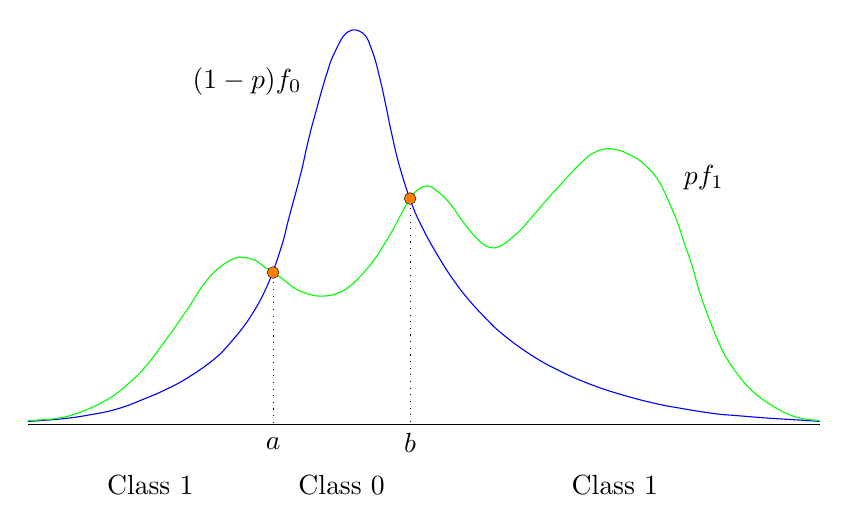
\begin{tikzpicture}
    % (1-p) f_0
    \draw [blue] plot[smooth, tension=.7] coordinates {
        (-4.88,-2.09) (-4.47,-2.06) (-4.11,-2.01) (-3.74,-1.93) (-3.37,-1.79)
        (-3.12,-1.68) (-2.86,-1.54) (-2.53,-1.31) (-2.32,-1.10) (-2.07,-0.78)
        (-1.85,-0.38) (-1.67, 0.11)  % first crossing (a)
        (-1.57, 0.49) (-1.42, 1.05) (-1.35, 1.36) (-1.29, 1.61) (-1.23, 1.83)
        (-1.15, 2.12) (-1.08, 2.35) (-1.00, 2.57) (-0.83, 2.85) (-0.63, 2.84)
        (-0.51, 2.61) (-0.42, 2.29) (-0.34, 1.93) (-0.27, 1.59)
        (-0.17, 1.17) (-0.02, 0.70)  % second crossing (b)
        ( 0.13, 0.36) ( 0.33, 0.00) ( 0.51,-0.28) ( 0.70,-0.53) ( 0.91,-0.76)
        ( 1.14,-0.98) ( 1.51,-1.25) ( 1.87,-1.45) ( 2.26,-1.62) ( 2.65,-1.75)
        ( 3.07,-1.86) ( 3.38,-1.92) ( 3.82,-1.99) ( 4.15,-2.02) ( 4.53,-2.05)
        ( 4.85,-2.07) ( 5.17,-2.09)
    };
    \node at (-2.10, 2.23) {$(1-p)f_{0}$};  % label

    % p f_1
    \draw [green] plot[smooth, tension=.7] coordinates {
        (-4.88,-2.08) (-4.70,-2.07) (-4.50,-2.05) (-4.29,-2.00) (-4.11,-1.93)
        (-3.94,-1.85) (-3.75,-1.73) (-3.55,-1.56) (-3.42,-1.43) (-3.29,-1.27)
        (-3.15,-1.08) (-3.04,-0.93) (-2.95,-0.80) (-2.84,-0.64) (-2.68,-0.39)
        (-2.56,-0.24) (-2.43,-0.12) (-2.26,-0.02) (-2.13,-0.01) (-1.99,-0.05)
        (-1.85,-0.15) (-1.69,-0.25)  % first crossing (a)
        (-1.51,-0.39) (-1.36,-0.46) (-1.18,-0.50) (-0.97,-0.47) (-0.79,-0.37)
        (-0.61,-0.19) (-0.48,-0.03) (-0.37, 0.14) (-0.25, 0.34) (-0.18, 0.47)
        (-0.07, 0.68) ( 0.02, 0.81)  % second crossing (b)
        ( 0.18, 0.90) ( 0.33, 0.82) ( 0.49, 0.66) ( 0.63, 0.46) ( 0.82, 0.23)
        ( 0.98, 0.12) ( 1.14, 0.15) ( 1.35, 0.32) ( 1.53, 0.52) ( 1.72, 0.74)
        ( 1.92, 0.96) ( 2.12, 1.17) ( 2.30, 1.32) ( 2.54, 1.37) ( 2.81, 1.27)
        ( 3.00, 1.12) ( 3.14, 0.94) ( 3.25, 0.71) ( 3.38, 0.40) ( 3.45, 0.18)
        ( 3.55,-0.11) ( 3.64,-0.43) ( 3.76,-0.77) ( 3.89,-1.09) ( 3.99,-1.29)
        ( 4.12,-1.48) ( 4.29,-1.68) ( 4.52,-1.86) ( 4.85,-2.03) ( 5.17,-2.08)
    };
    \node at ( 3.70, 1.01) {$pf_{1}$};  % label

    % first crossing (a)
    \draw (-1.77,-0.20) node (a) {} circle (2pt);  % circle (a)
    \fill [orange, thick] (a) circle (2pt);         % fill circle
    \draw [dotted] (a) -- (-1.77,-2.13);           % dotted line to x-axis
    \node at (-1.77,-2.37) {$a$};                  % label on x-axis

    % second crossing (b)
    \draw (-0.03, 0.74) node (b) {} circle (2pt);  % circle (b)
    \fill [orange, thick] (b) circle (2pt);        % fill circle
    \draw [dotted] (b) -- (-0.03,-2.13);           % dotted line to x-axis
    \node at (-0.03,-2.37) {$b$};                  % label on x-axis

    % x-axis & class labels
    \draw (-4.88,-2.13) -- ( 5.17,-2.13);  % x-axis
    \node at (-3.33,-2.90) {Class 1};      % (-\infty, a)
    \node at (-0.90,-2.90) {Class 0};      % [a, b]
    \node at ( 2.57,-2.90) {Class 1};      % (b, \infty)
\end{tikzpicture}
}
    \caption{%
        Illustration of the Bayes classifier in case the distribution of $X$ is given by a density $f$ and conditional densities $f_0$ and $f_1$ exist. The classifier equals $0$ on the interval $[a, b]$ and $1$ elsewhere.
    }
\end{figure}
If we additionally assume that both classes are equally likely, i.e., $p = 1-p = 1/2$, the Bayes classifier becomes
\[
    h^*(x) = \begin{cases}
        1, \quad & f_1(x) > f_0(x) \\
        0, \quad &\text{else}
    \end{cases}
\]
and its error is given by
\[
    L^* = \frac{1}{2} \int_{\mathcal{X}} \min(f_1(x), f_0(x)) \dx = \frac{1}{2} \int_{\mathcal{X}} f_1(x) - (f_1(x) - f_0(x))^+ \dx = \frac{1}{2} - \frac{1}{4} \int_{\mathcal{X}} \bigAbs{ f_1(x) - f_0(x) } \dx \, ,
\]
where $g^+ = \max(g, 0)$ denotes the positive part of a function $g$. This demonstrates that the Bayes error is directly related to the $L^1$-distance between the class densities $f_1$ and $f_0$.

%% SECTION 2.2 %%
\section{Plug-In Decisions}
\label{subsec: plug-in decisions}

We know that the Bayes classifier $h^*(x) = \indSet{\eta(X) > 1/2}$ is our best guess of $Y$ based on the observation $X$. However, the function $\eta(x) = \Ex{Y \given X=x}$ is often unknown. Assume that we have a function $\tilde\eta \colon \mathcal{X} \to [0, 1]$ approximating $\eta$. In this case, it is natural to use the \emph{plug-in} decision function
\begin{equation}
\label{eq: plug-in classifier}
    \tilde h(x) = \begin{cases}
        1, \quad &\tilde\eta(x) > 1/2 \\
        0, \quad &\tilde\eta(x) \leq 1/2
    \end{cases}
\end{equation}

The error probability of this plug-in classifier is close to the optimal classifier $h^*$.

\begin{theorem}
\label{thm: plug-in decision}
The excess risk $R(\tilde h)$ of the plug-in classifier $\tilde h$ defined in \eqref{eq: plug-in classifier} satisfies
\[
    R(\tilde h) = \ex{\abs{2 \eta(X) - 1} \cdot \indSet{\tilde h(X) \neq h^*(X)}} \leq 2 \, \Ex{\bigAbs{ \eta(X) - \tilde\eta(X) }}.
\]
\end{theorem}

\begin{proof}
The first identity is simply an application of Theorem \ref{thm: bayes classifier}. Thus, all we need to demonstrate is that the inequality
\[
    \bigAbs{ \eta(x) - 1/2 } \leq \bigAbs{ \eta(x) - \tilde\eta(x) }
\]
holds on the set $A = \{\tilde h \neq h^*\}$. First, assume that $\tilde h(x) = 0$ for $x \in A$. This implies that $h^*(x) = 1$. By definition of $\tilde h$ and $h^*$, we know that $\tilde\eta(x) \leq 1/2$ and $\eta(x) > 1/2$, and thus
\[
    \tilde\eta(x) \leq 1/2 < \eta(x).
\]
If $\tilde h(x) = 1$, then $h^*(x) = 0$, and consequently $\tilde\eta(x) > 1/2$ and $\eta(x) \leq 1/2$. Altogether, we have
\[
    \eta(x) \leq 1/2 < \tilde\eta(x).
\]
This proves the inequality stated at the beginning of this proof.
\end{proof}

Since $\eta \colon \mathcal{X} \to [0, 1]$ takes values in the unit interval, the condition $\eta(x) > 1/2$ is equivalent to the inequality $\eta(x) > 1 - \eta(x)$. Assuming that we have two functions $\tilde\eta_1 \colon \mathcal{X} \to [0, 1]$ and $\tilde\eta_0 \colon \mathcal{X} \to [0, 1]$ such that $\tilde\eta_1$ approximates $\eta$ and $\tilde\eta_0$ approximates $1 - \eta$ with the constraint that $\tilde\eta_1$ and $\tilde\eta_0$ do \emph{not} sum to $1$, we can still build a plug-in classifier $\tilde h$ by plugging $\tilde\eta_1$ and $\tilde\eta_0$ into the condition $\eta(x) > 1 - \eta(x)$:
\begin{equation}
\label{eq: plug-in classifier not summing to 1}
    \tilde h(x) = \begin{cases}
        1, \quad &\tilde\eta_1(x) > \tilde\eta_0(x) \\
        0, \quad &\text{else}
    \end{cases}
\end{equation}
While this puts us into a slightly different situation compared to Theorem \ref{thm: plug-in decision}, a bound similar to that in Theorem \ref{thm: plug-in decision} still holds.

\begin{theorem}
The excess risk $R(\tilde h)$ of the plug-in classifier $\tilde h$ defined in \eqref{eq: plug-in classifier not summing to 1} satisfies
\[
    R(\tilde h) \leq \Ex{\abs{\eta(X) - \tilde{\eta}_1(X)}} + \Ex{\abs{(1 - \eta(X)) - \tilde{\eta}_0(X)}}.
\]
\end{theorem}

The proof is left to the reader. Finally, assume that the class-conditional densities $f_0$ and $f_1$ exist and are approximated by $\tilde f_0$ and $\tilde f_1$. Further, let the class probabilities $p = \Pr{Y=1}$ and $1-p = \Pr{Y=0}$ be approximated by $\tilde p_1$ and $\tilde p_0$, respectively. In this case, one might use the plug-in decision
\begin{equation}
\label{eq: plug-in classifier for X with density}
    \tilde h(x) = \begin{cases}
        1, \quad &\tilde f_1(x) \tilde p_1 > \tilde f_0(x) \tilde p_0 \\
        0, \quad &\text{else}
    \end{cases}
\end{equation}
which is based on the Bayes classifier established in \eqref{eq: bayes classifier for X with density}.

\begin{proposition}
The excess risk $R(\tilde h)$ of the plug-in classifier $\tilde h$ defined in \eqref{eq: plug-in classifier for X with density} satisfies
\[
    R(\tilde h) \leq \int_{\mathcal{X}} \bigAbs{ p f_1(x) - \tilde p_1 \tilde f_1(x) } \dx + \int_{\mathcal{X}} \bigAbs{ (1-p) f_0(x) - \tilde p_0 \tilde f_0(x) } \dx \, .
\]
\end{proposition}

The proof is left to the reader once again.

%% SECTION 2.3 %%
\section{Empirical Classification}
\label{subsec: empirical classification}

In reality, we do \emph{not} know the true distribution of $(X, Y)$. Instead, we are often working with finite sets of data $\mathcal{D}_n = \set{(X_1, Y_1), \dots, (X_n, Y_n)}$ (e.g., a training set), where the $(X_i, Y_i)$ are (hypothetical) \emph{future} i.i.d. draws from $\P_{(X, Y)}$. Note that, if we build a classifier $h_n(X)$ based on this data, the classifier is random in two senses: it is a function of a random variable $X$, and it depends implicitly on the random data $\mathcal{D}_n$. Further, the error probability
\[
    L(h_n) = \P(h_n (X) \neq Y)
\]
is a \emph{random variable}, as it depends on the random data $\mathcal{D}_n$! Nevertheless, the excess risk
\[
    R(h_n) = L(h_n) - L^* \geq 0
\]
is always non-negative (in a deterministic sense, \emph{not} only almost surely). One approach of building a classifier based on the observed data $\mathcal{D}_n$ is the following: based on the observations $(X_1, Y_1), \dots, (X_n, Y_n)$, we estimate $\eta$ by $\eta_n$ and then construct the plug-in classifier $h_n = \indSet{\eta_n > \nicefrac{1}{2}}$. However, the (true) excess risk of $h_n$ is \emph{not} computable based on the data alone and we cannot use any results for upper bounds on the excess risk $R(h_n)$ discussed in Section \ref{subsec: plug-in decisions}. A naive attempt to solve this problem is the definition of \emph{empirical risk}, which essentially replaces the expected deviation of $h_n(X)$ from $Y$ by a simple average:

\begin{definition}
The \emph{empirical risk} of a classifier $h$ with respect to the data $\mathcal{D}_n$ is given by
\[
    \hat L_n(h) = \frac{1}{n} \sum_{i=1}^n \indSet{h(X_i) \neq Y_i}.
\]
\end{definition}

The empirical risk $\hat L_n(h)$ of a classifier $h$ is an \emph{unbiased estimator} of its true risk $L(h)$, i.e.,
\begin{equation}
\label{eq: bias of empirical risk}
    \highlightMath{
        \Ex{\hat L_n(h)} = \frac{1}{n} \sum_{i=1}^n \Ex{\indSet{h(X_i) \neq Y_i}} = \frac{1}{n} \sum_{i=1}^n \Pr{h(X_i) \neq Y_i} = \Pr{h(X) \neq Y} = L(h),
    }
\end{equation}
since $(X_i, Y_i)$ are i.i.d. draws from the distribution of $(X, Y)$.

Minimizing the empirical risk over all classifiers is useless since, for every hypothetical data set, we can always construct a classifier with \emph{no} empirical risk by just mimicking the data and classifying arbitrarily otherwise, i.e., the classifier
\[
    h_n(x) = \begin{cases}
        1, \quad &x = X_i \text{ for some } i = 1, \dots, n \text{ with } Y_i = 1 \\
        0, \quad &x = X_i \text{ for some } i = 1, \dots, n \text{ with } Y_i = 0 \\
        a, \quad &x \notin \set{X_1, \dots, X_n}
    \end{cases}
\]
with $a \in \set{0, 1}$ arbitrary, satisfies $\hat L_n(h_n) = 0$. Thus, we have to restrict ourselves to classifiers in a certain family $\mathcal{H}$.

\begin{definition}
The \emph{empirical risk minimizer} over $\mathcal{H}$ is any element $\hat h^{\text{erm}}$ of the set $\argmin_{h \in \mathcal{H}} \hat L_n(h)$, i.e., $\hat h^{\text{erm}} \in \mathcal{H}$ and $\hat L_n(\hat h^{\text{erm}}) = \min_{h \in \mathcal{H}} \hat L_n(h)$.
\end{definition}

For meaningful results, $\mathcal{H}$ should be much smaller than the set of all classifiers. On the other hand, $\mathcal{H}$ should not be \emph{too} small, because we want the empirical risk of $\hat h^{\text{erm}}$ to be close to the Bayes risk. Often, we will be satisfied with a classifier $\hat h$ that is reasonably close to the empirical risk minimizer $\hat h^{\text{erm}}$ in the sense that
\[
    \hat L_n(\hat h) \leq \min_{h \in \mathcal{H}} \hat L_n(h) + \varepsilon, \quad \text{for small } \varepsilon > 0.
\]
Given a family $\mathcal{H}$, let $\bar h$ be a classifier that somehow minimizes the \emph{true} risk, i.e.,
\[
    \highlightMath{
        \bar h \in \argmin_{h\in \mathcal{H}} L(h).
    }
\]
Note that it is impossible to construct such a classifier -- often called an \emph{oracle} -- from data alone. Nonetheless, we can attempt to find a classifier $\hat h$ that mimics the performance of the oracle $\bar h$ in the sense that we can hope to prove a bound of the form
\begin{equation}
    \label{eq: oracle inequality}
    L(\hat h) \leq L(\bar h) + \text{something small}.
\end{equation}
Such inequalities are often called \emph{oracle inequalities} as they involve the oracle $\bar h$. In \eqref{eq: oracle inequality}, we once again see the trade-off regarding the size of $\mathcal{H}$. If $\mathcal{H}$ is small, the performance of the oracle $\bar h$ is likely to suffer, while it might be possible to approximate $\bar h$ quite closely. If, on the other hand, $\mathcal{H}$ is quite large, the oracle $\bar h$ will be very powerful, but approximating $\bar h$ becomes statistically more difficult.

Ultimately\footnote{Remember that $L(\hat f)$ is a random variable!}, we want to prove tail bounds or bounds in expectation of the form
\[
    \Pr{L(\hat h) \leq L(\bar h) + \Delta_{n, \delta}(\mathcal{H})} \geq 1 - \delta,
\]
where $\Delta_{n, \delta}(\mathcal{H})$ is some function of $\mathcal{H}$ depending on our sample size $n$ and our desired level of confidence $\delta$.

Finally, note that we can decompose the excess risk $R(\hat h)$ of a classifier as follows:
\[
    \highlightMath{
        R(\hat h) = L(\hat h) - L^* = \underbrace{L(\hat h) - L(\bar h)}_{\substack{\text{estimation} \\ \text{error}}} + \underbrace{L(\bar h) - L^*}_{\substack{\text{approximation} \\ \text{error}}}
    }
\]
The second term is the \emph{approximation error} that is unavoidable once we fix a family of classifiers $\mathcal{H}$. Oracle inequalities provide a method to bound the first term, the \emph{estimation error}.

%% SECTION 2.4 %%
\section{Hoeffding's Inequality}

An important technique for understanding the empirical error and classifiers based on the empirical distribution are so-called \emph{concentration inequalities}, which we will consider in more detail later. These are results that allow us to bound the deviations of a function of random variables from some value (often, its mean). Two very simple inequalities are the following:

\begin{prop}
\begin{itemize}
    \item \emph{Markov's inequality}: $\Pr{X \geq t} \leq \nicefrac{\Ex{X}}{t}$ for $X \geq 0$ and $t > 0$,

    \item \emph{Chebyshev’s inequality}: $\Pr{\abs{X - \Ex{X}} \geq t} \leq \nicefrac{\Var(X)}{t^2}$ for $X$ with $\Var(X) < \infty$ and $t > 0$.
\end{itemize}
\end{prop}

\noindent The main result of this section is \emph{Hoeffding's inequality}, which we will subsequently apply in order to bound the estimation error $L(\hat h) - L(\bar h)$ (see Theorem \ref{thm: estimation error finite dictionary}).

To prove Hoeffding's inequality, we will have to control the moment-generating function\footnote{Recall that the moment-generating function of a random variable $X$ is defined as $M_X(s) = \Ex{\e^{sX}}$. Its name reflects the fact that the $n$-th moment of $X$ (given that it exists) can be obtained by evaluating the $n$-th derivative of $M_X$ at $s=0$.} of a bounded random variable. Hence, we start with the following lemma:

\begin{lemma}[Hoeffding's Lemma]
\label{lem: hoeffding}
Let $X$ be a random variable satisfying $a \leq X \leq b$ almost surely. Then, 
the moment-generating function of $X - \Ex{X}$ satisfies
\[
    \Ex{\e^{s(X - \Ex{X})}} \leq \exp(\frac{s^2(b-a)^2}{8}).
\]
\end{lemma}

\begin{proof}
Write $\mu = \Ex{X}$, and let $Z = X - \mu$, so that $\Ex{Z} = 0$ and $a - \mu \leq Z \leq b - \mu$. It suffices to prove that the \emph{cumulant-generating function} $\psi(s) = \log\Ex{\e^{sZ}}$ satisfies
\[
    \psi(s) \leq \frac{s^2(b-a)^2}{8}.
\]
We can interchange the order of differentiation and integration since $Z$ is bounded. Doing so yields
\[
    \psi'(s) = \frac{\Ex{Z\e^{sZ}}}{\Ex{\e^{sZ}}}
\]
and
\[
    \psi''(s) = \frac{\Ex{Z^2\e^{sZ}} \Ex{\e^{sZ}} - \Ex{Z\e^{sZ}}^2}{\Ex{\e^{sZ}}^2} = \Ex{Z^2 \frac{\e^{sZ}}{\Ex{\e^{sZ}}}} - \left(\Ex{Z \frac{\e^{sZ}}{\Ex{\e^{sZ}}}}\right)^2.
\]
Since the term $\frac{\e^{sZ}}{\Ex{\e^{sZ}}}$ integrates to $1$, we can interpret $\psi''(s)$ as the variance of $Z$ with respect to the measure $\mathrm{d}\mathbb{Q} = \frac{\e^{sZ}}{\Ex{\e^{sZ}}} \mathrm{d}\P$, i.e.,
\[
    \psi''(s) = \mathbb{E}_{\mathbb{Q}}[Z^2] - \mathbb{E}_{\mathbb{Q}}[Z]^2 = \mathrm{Var}_{\mathbb{Q}}(Z) = \mathrm{Var}_{\mathbb{Q}}\left(Z + \mu - \frac{a+b}{2}\right).
\]
The last identity in the previous computation holds since the variance of a random variable is not affected by constant shifts. From $Z + \mu \in [a,b]$ almost surely, it follows that $\abs{Z + \mu - \frac{a+b}{2}} \leq \frac{b-a}{2}$ almost surely, and hence
\[
    \psi''(s) = \mathrm{Var}_{\mathbb{Q}}\left(Z + \mu - \frac{a+b}{2}\right) \leq \mathbb{E}_{\mathbb{Q}}\left[\left(Z + \mu - \frac{a+b}{2}\right)^2\right] \leq \frac{(b-a)^2}{4}.
\]
Finally, the fundamental theorem of calculus yields
\[
    \psi(s) = \int_0^s\int_0^u \psi''(v) \, \mathrm{d}v \, \mathrm{d}u \leq \frac{(b-a)^2}{4} \int_0^s u \, \mathrm{d}u = \frac{(b-a)^2}{4} \frac{s^2}{2} = \frac{s^2(b-a)^2}{8},
\]
concluding the proof.
\end{proof}

Equipped with this result, we can tackle Hoeffding's inequality:

\begin{theorem}[Hoeffding, 1963]
\label{thm: hoeffding}
Let $X_1, \dots, X_n$ be independent random variables such that, almost surely, $a_i \leq X_i \leq b_i$, and denote the sum of the $X_i$ by $S_n = \sum_{i=1}^n X_i$. Then, for any $t>0$,
\[
    \Pr{\abs{S_n - \Ex{S_n}} \geq t} \leq 2 \exp(\frac{-2t^2}{\sum_{i=1}^n (b_i - a_i)^2}).
\]
\end{theorem}

\begin{proof}
It suffices to show the inequality
\[
    \Pr{S_n - \Ex{S_n} \geq t} \leq \exp(\frac{-2t^2}{\sum_{i=1}^n (b_i - a_i)^2})
\]
as the bound for the lower tail follows analogously. For any $s>0$, we have
\[
    \Pr{S_n - \Ex{S_n} \geq t} = \Pr{\exp(s(S_n - \Ex{S_n})) \geq \exp(st)} \leq \exp(-st) \Ex{\exp(s(S_n - \Ex{S_n}))},
\]
where we have applied Markov's inequality\footnote{This is what is referred to as the \emph{generic Chernoff bound}, which -- for a random variable $X$ -- is attained by applying Markov's inequality to $\e^{tX}$ with $t > 0$. Doing so yields $\Pr{X \geq a} = \Pr{\e^{tX} \geq \e^{ta}} \leq \e^{-ta} \Ex{e^{tX}} = \e^{-ta} M_X(t)$.}. Since the $X_i$ are independent, we have
\[
    \Ex{\exp(s(S_n - \Ex{S_n}))} = \Ex{\exp(\sum_{i=1}^n s(X_i - \Ex{X_i}))} = \prod_{i=1}^n \Ex{\exp(s(X_i - \Ex{X_i}))},
\]
and hence, by Hoeffding's lemma,
\[
    \exp(-st) \prod_{i=1}^n \Ex{\exp(s(X_i - \Ex{X_i}))} \leq \exp(-st) \prod_{i=1}^n \exp(\frac{s^2 (b_i-a_i)^2}{8}) = \exp(-st + \frac{s^2}{8} \sum_{i=1}^n (b_i-a_i)^2).
\]
To optimize the bound, we want to minimize the expression inside the exponential function. For ease of notation, let $\lambda = \sum_{i=1}^n (b_i-a_i)^2$. With this notation, differentiating $f(s) = \frac{\lambda}{8} s^2 -ts$ and subsequently setting it equal to $0$ gives
\[
    \frac{\lambda}{4} s - t = 0,
\]
which yields the optimal solution $s^* = \frac{4t}{\lambda}$. Hence, the best bound we can find is
\[
    \exp(f(s^*)) = \exp(\frac{\lambda}{8} \left(\frac{4t}{\lambda}\right)^2 - t \frac{4t}{\lambda}) = \exp(\frac{-2t^2}{\lambda}) = \exp(\frac{-2t^2}{\sum_{i=1}^n (b_i - a_i)^2}),
\]
which is exactly the upper bound we wanted to prove.
\end{proof}

\begin{remark}
Let $X_1, \dots, X_n$ be random variables satisfying the conditions of Theorem \ref{thm: hoeffding}, and write $\bar X = S_n/n$ for the arithmetic mean of the $X_i$. We have
\[
    \Pr{\abs{\bar X - \ex{\bar X}} \geq t} = \Pr{\abs{S_n - \Ex{S_n}} \geq nt} \leq 2 \exp(\frac{-2n^2t^2}{\sum_{i=1}^n (b_i - a_i)^2}).
\]
Further, observe that the expression $\bar X - \ex{\bar X}$ can be rewritten as $\frac{1}{n} \sum_{i=1}^n (X_i - \Ex{X_i})$. Hence, Hoeffding's inequality ensures that the (absolute) average deviation of independent and (almost surely) bounded random variables from their respective means decays \emph{exponentially fast} in the number of observations $n$. Finally, if the random variables $X_1, \dots, X_n$ are i.i.d. random variables such that, almost surely, $a \leq X_i \leq b$, Hoeffding's inequality states that
\[
    \Pr{\abs{\bar X - \ex{X_1}} \geq t} \leq 2 \exp(\frac{-2nt^2}{(b - a)^2}).
\]
For random variables $X_i$ taking values in the unit interval, this reduces to
\[
    \Pr{\abs{\bar X - \ex{X_1}} \geq t} \leq 2 \e^{-2nt^2}.
\]
\end{remark}

%% SECTION 2.5 %%
\section{Learning with a Finite Dictionary}

Recall the setup of Section \ref{subsec: empirical classification}: given a family $\mathcal{H}$ of classifiers, we want to bound the estimation error $L(\hat h) - L(\bar h)$, where
\[
    \hat h \in \argmin_{h \in \mathcal{H}} \hat L_n(h)
\]
is the empirical risk minimizer, which minimizes the \emph{empirical} risk over $\mathcal{H}$, and
\[
    \bar h \in \argmin_{h \in \mathcal{H}} L(h)
\]
is the oracle, which minimizes the \emph{true} risk over the family $\mathcal{H}$. Keep in mind that the empirical risk minimizer $\hat h$ is a random variable that depends on the random data $\mathcal{D}_n$. In this section, we will prove a bound on the estimation error $L(\hat h) - L(\bar h)$ under the assumption that the family $\mathcal{H} = \set{h_1, \dots, h_M}$ is a \emph{finite} set of classifiers. In particular, we want to better understand the scaling of the estimation error with respect to the number $M$ of classifiers and the number $n$ of observations.

To get started, observe that the estimation error satisfies
\[
    L(\hat h) - L(\bar h) = \left(L(\hat h) - \hat L_n(\bar h)\right) + \left(\hat L_n(\bar h) - L(\bar h)\right) \leq \left(L(\hat h) - \hat L_n(\hat h)\right) + \left(\hat L_n(\bar h) - L(\bar h)\right),
\]
since $\hat L_n(\hat h) \leq \hat L_n(\bar h)$ by definition of the empirical risk minimzer. Thus, we can find a bound on the estimation error by bounding the deviation of the empirical risk $\hat L_n(h)$ of a classifier $h$ from its true risk $L(h)$. This is where Hoeffding's inequality comes in handy.

\begin{theorem}
\label{thm: empirical vs true risk}
\begin{enumerate}[(i)]
    \item For a classifier $h$ and $\delta > 0$,
    \[
        \Pr{\bigAbs{ \hat L_n(h) - L(h) } < \sqrt{\frac{\log(2/\delta)}{2n}}} \geq 1 - \delta.
    \]

    \item If $\mathcal{H} = \set{h_1, \dots, h_M}$ is a \emph{finite} family of $M$ classifiers, then
    \[
        \Pr{\max_{h \in \mathcal{H}} \bigAbs{ \hat L_n(h) - L(h) } < \sqrt{\frac{\log(2M/\delta)}{2n}}} \geq 1 - \delta.
    \]
\end{enumerate}
\end{theorem}

\begin{proof}
Since $(X_i, Y_i)$ are i.i.d. draws from $\P_{(X, Y)}$, we have
\[
    \Pr{h(X) \neq Y} = \Ex{\indSet{h(X) \neq Y}} = \frac{1}{n} \sum_{i=1}^n \Ex{\indSet{h(X) \neq Y}} = \frac{1}{n} \sum_{i=1}^n \Ex{\indSet{h(X_i) \neq Y_i}},
\]
and hence,
\[
    \hat L_n(h) - L(h) = \frac{1}{n} \sum_{i=1}^n \indSet{h(X_i) \neq Y_i} - \Ex{\indSet{h(X_i) \neq Y_i}}.
\]
The first assertion thus follows from Hoeffding's inequality applied to the random variables $\indSet{h(X_i) \neq Y_i}$, $i = 1, \dots, n$ and $t = \sqrt{\frac{\log(2/\delta)}{2n}}$, since $\Pr{\abs{\ldots} < t} = 1 - \Pr{\abs{\ldots} \geq t} \geq 1 - 2\e^{-2nt^2} = 1 - \delta$.

For the second assertion, observe that, for $t = \sqrt{\frac{\log(2M/\delta)}{2n}}$,
\[
    \set{\max_{h \in \mathcal{H}} \bigAbs{ \hat L_n(h) - L(h) } \geq t} = \bigcup_{j=1}^M \set{\bigAbs{ \hat L_n(h_j) - L(h_j) } \geq t}
\]
and hence,
\[
    \Pr{\max_{h \in \mathcal{H}} \bigAbs{ \hat L_n(h) - L(h) } < t} = 1 - \Pr{\max_{h \in \mathcal{H}} \bigAbs{ \hat L_n(h) - L(h) } \geq t} \geq 1 - \sum_{j=1}^M \Pr{\bigAbs{ \hat L_n(h_j) - L(h_j) } \geq t}
\]
by applying a simple union bound. As before, Hoeffding's inequality yields
\[
    \Pr{\bigAbs{ \hat L_n(h_j) - L(h_j) } \geq t} \leq 2\e^{-2nt^2} = \frac{\delta}{M}, \quad j = 1, \dots, M.
\]
Putting everything together, we obtain
\[
    \Pr{\max_{h \in \mathcal{H}} \bigAbs{ \hat L_n(h) - L(h) } < t} \geq 1 - \sum_{j=1}^M \Pr{\bigAbs{ \hat L_n(h_j) - L(h_j) } \geq t} \geq 1 - \sum_{j=1}^M \frac{\delta}{M} = 1 - \delta.
\]
\end{proof}

As hinted at before, we can now use this intermediate result to obtain a bound on the estimation error $L(\hat h) - L(\bar h)$. Loosely speaking, while the empirical risk minimizer $\hat h$ generally performs worse (in terms of the true risk) than the oracle $\bar h$, their difference is not too big, given that the sample size $n$ is large enough compared to the number $M$ of classifiers in $\mathcal{H}$.

\begin{theorem}
\label{thm: estimation error finite dictionary}
For a finite family of classifiers $\mathcal{H} = \set{h_1, \dots, h_M}$ and $\delta > 0$, the estimation error $L(\hat h) - L(\bar h)$ satisfies
\[
    \Pr{L(\hat h) - L(\bar h) < \sqrt{\frac{2\log(2M/\delta)}{n}}} \geq 1 - \delta.
\]
\end{theorem}

\begin{proof}
We have
\[
    L(\hat h) - L(\bar h) = \left(L(\hat h) - \hat L_n(\bar h)\right) + \left(\hat L_n(\bar h) - L(\bar h)\right) \leq \left(L(\hat h) - \hat L_n(\hat h)\right) + \left(\hat L_n(\bar h) - L(\bar h)\right),
\]
since $\hat L_n(\hat h) \leq \hat L_n(\bar h)$ by definition of the empirical risk minimzer. Since we do not have any information about the oracle $\bar h$, we bound both terms of the RHS by a maximum over $\mathcal{H}$:
\[
    \left(L(\hat h) - \hat L_n(\hat h)\right) + \left(\hat L_n(\bar h) - L(\bar h)\right) \leq 2 \max_{j} \bigAbs{ \hat L_n(h_j) - L(h_j) }.
\]
Summarizing, we have
\[
    L(\hat h) - L(\bar h) \leq 2 \max_j \bigAbs{ \hat L_n(h_j) - L(h_j) },
\]
and thus, Theorem \ref{thm: empirical vs true risk} implies
\begin{align*}
    \Pr{L(\hat h) - L(\bar h) < \sqrt{\frac{2\log(2M/\delta)}{n}}} &\geq \Pr{2 \max_j \bigAbs{ \hat L_n(h_j) - L(h_j) } < \sqrt{\frac{2\log(2M/\delta)}{n}}} \\
        &= \Pr{\max_j \bigAbs{ \hat L_n(h_j) - L(h_j) } < \sqrt{\frac{\log(2M/\delta)}{2n}}} \geq 1 - \delta.
\end{align*}
\end{proof}

Let us make a few remarks before we move on. First, the parameter $\delta > 0$ allows us to control the confidence we want to have in the bound on the estimation error. Here, we see a typical trade-off: for smaller $\delta$, the bound on the estimation error becomes less restrictive, but at the same time, the probability that the bound actually holds, increases (and vice versa). Further, for fixed $\delta$, the bound becomes sharper as the number $n$ of observations increases and the number $M$ of classifiers decreases.


%% CHAPTER 3 %%
\chapter{Concentration Inequalities}

Concentration inequalities are results that allow us to bound the deviations of a function of random variables from its mean. The first inequality we will consider improves on Hoeffding's inequality by allowing for some dependence between the random variables.

%% SECTION 3.1 %%
\section{Azuma-Hoeffding Inequality}

To state the main result of this section, we first need to introduce the concept of \emph{martingales}.

\begin{definition}
Let $(\Omega, \mathcal{A}, \mathbb{P})$ be a probability space.
\begin{enumerate}[(i)]
    \item A \emph{filtration} $\set{\mathcal{F}_n}_{n \in \N}$ is an increasing sequence of sub-$\sigma$-algebras $\mathcal{F}_n$ of $\mathcal{A}$, i.e.,
    \[
        \mathcal{F}_1 \subseteq \mathcal{F}_2 \subseteq \dots \subseteq \mathcal{A}.
    \]

    \item A stochastic process $\set{X_n}_{n \in \N}$ is called a \emph{martingale} if, for every $n \in \N$,
    \begin{enumerate}[(a)]
        \item $X_n$ is $\mathcal{F}_n$-measurable and integrable, i.e., $\Ex{\abs{X_n}} < \infty$,

        \item $\Ex{X_{n+1} \given \mathcal{F}_n} = X_n$ holds almost surely.
    \end{enumerate}
\end{enumerate}
\end{definition}

Loosely speaking, martingales are a generalization of sums of zero-mean, independent random variables: Let $\set{X_n}_{n \in \N}$ be a sequence of independent random variables with $\Ex{X_n} = 0$, and let $S_n = \sum_{i=1}^n X_i$. Then, for $\mathcal{F}_n = \sigma(X_1, \dots, X_n)$, we have
\[
    \Ex{S_{n+1} \given \mathcal{F}_n} = \Ex{X_{n+1} + S_n \given \mathcal{F}_n} = \Ex{X_{n+1}} + \Ex{S_n \given \mathcal{F}_n} = S_n,
\]
since $X_{n+1}$ is centered and independent of $\mathcal{F}_n$, and $S_n$ is $\mathcal{F}_n$-measurable.

Another definition we will need is that of a \emph{martingale difference sequence}.

\begin{definition}
Let $(\Omega, \mathcal{A}, \mathbb{P})$ be a probability space with filtration $\set{\mathcal{F}_n}_{n \in \N}$. A stochastic process $\set{X_n}_{n\in\N}$ is called a \emph{martingale difference sequence (MDS)}, if
\begin{enumerate}[(i)]
    \item $X_n$ is $\mathcal{F}_n$-measurable and integrable, i.e., $\Ex{\abs{X_n}} < \infty$,

    \item $\Ex{X_{n+1} \given \mathcal{F}_n} = 0$ holds almost surely.
\end{enumerate}
\end{definition}

Whenever we have a martingale $\set{X_n}_{n\in\N}$, we can construct a martingale difference sequence by setting $\Delta_n = X_n - X_{n-1}$, since then
\[
    \Ex{\Delta_{n+1} \given \mathcal{F}_n} = \Ex{X_{n+1} - X_n \given \mathcal{F}_n} = \Ex{X_{n+1} \given \mathcal{F}_n} - X_n = 0.
\]

\begin{theorem}[Azuma-Hoeffding]
\label{thm: azuma-hoeffding}
Assume that $\set{\Delta_i}_{i\in\N}$ is a martingale difference sequence with respect to a filtration $\set{\mathcal{F}_i}_{i\in\N}$ and let $A_i, B_i$ be $\mathcal{F}_i$-measurable random variables such that
\[
    A_i \leq \Delta_i \leq B_i
\]
holds almost surely for all $i \in \N$. Then,
\[
    \Pr{\frac{1}{n}\sum_{i=1}^n \Delta_i \geq t} \leq \exp(\frac{-2n^2t^2}{\sum_{i=1}^n \norm{A_i - B_i}_\infty^2})
\]
\end{theorem}

In comparison to Hoeffding’s inequality, the Azuma-Hoeffding inequality allows for non-uniform boundedness and does not require independence of the random variables.

\begin{proof}
As in the proof of Hoeffding's inequality, we first apply the generic Chernoff bound to obtain
\begin{align*}
    \Pr{\frac{1}{n}\sum_{i=1}^n \Delta_i \geq t} \leq \Ex{\e^{s\sum_i \Delta_i}} \e^{-snt} &= \Ex{\Ex{\e^{s\sum_i \Delta_i} \given \mathcal{F}_{n-1}}} \e^{-snt} \\
        &= \Ex{\e^{s\sum_{i=1}^{n-1} \Delta_i} \Ex{\e^{s\Delta_n} \given \mathcal{F}_{n-1}}} \e^{-snt}.
\end{align*}
Next, we apply Hoeffding's lemma to the inner expectation $\Ex{\e^{s\Delta_n} \given \mathcal{F}_{n-1}}$ to obtain
\begin{align*}
    \Pr{\frac{1}{n}\sum_{i=1}^n \Delta_i \geq t} &\leq \Ex{\e^{s\sum_{i=1}^{n-1} \Delta_i} \e^{s^2\frac{(B_n - A_n)^2}{8}}} \e^{-snt} \\
        &\leq \Ex{\e^{s\sum_{i=1}^{n-1} \Delta_i}} \exp(\frac{s^2}{8}\norm{A_n - B_n}^2_\infty) \e^{-snt}.
\end{align*}
Iteratively splitting off the $\Delta_i$ one-by-one and then applying Hoeffding's lemma, we eventually get
\[
    \Pr{\frac{1}{n}\sum_{i=1}^n \Delta_i \geq t} \leq \exp(\frac{s^2}{8}\sum_{i=1}^n \norm{A_i - B_i}_\infty^2) \e^{-snt}.
\]
As usual, optimizing the RHS over $s$ yields the desired result.
\end{proof}

%% SECTION 3.2 %%
\section{Bounded Differences Inequality}

Although the Azuma-Hoeffding Inequality is a strong result, it can be challenging to apply to a specific problem, and its complete usefulness is often wasted. Thankfully, there is a natural choice of the filtration $\set{\mathcal{F}_i}_{i \in \N}$ and the MDS $\set{\Delta_i}_{i \in \N}$ that provides an equally potent result that is easier to use. Before we can state said result, we need to introduce yet another definition.

\begin{definition}
A function $g \colon \mathcal{X}_1 \times \dots \times \mathcal{X}_n \to \R$ satisfies the \emph{bounded differences condition for constants $c_1, \dots, c_n \in \R$}, if the inequality
\[
    \sup_{\tilde{x}_i \in \mathcal{X}_i} \abs{g(x_1, \dots, x_n) - g(x_1, \dots, \tilde{x}_i, \dots, x_n)} \leq c_i
\]
holds for all $i = 1, \dots, n$ and all $x_1 \in \mathcal{X}_1, \dots, x_n \in \mathcal{X}_n$.
\end{definition}

Intuitively, $g$ meets the bounded differences condition if changing only one coordinate of $g$ at a time cannot cause the value of $g$ to deviate too far. For example, the empirical risk $\hat{L}_n(h) = \frac{1}{n} \sum_{i=1}^n \indSet{h(X_i) \neq Y_i}$ of a classifier $h$ satisfies the bounded differences condition for $c_i = \frac{1}{n}$. Similarly, the empirical mean $\frac{1}{n} \sum_{i=1}^n X_i$ of bounded random variables $X_i \in (a_i, b_i)$ satisfies the bounded differences inequality for $c_i = b_i - a_i$. It is not too surprising that these types of functions concentrate somewhat strongly around their average, and this intuition is made precise by the following result.

\begin{theorem}[Bounded Differences Inequality {[McDiarmid, 1989]}]
\label{thm: bounded differences inequality}
Let $X_1, \dots, X_n$ be independent random variables and let $g \colon \mathcal{X}_1 \times \dots \times \mathcal{X}_n \to \R$ be a function satisfying the bounded differences condition for constants $c_1, \dots, c_n \in \R$. Then,
\[
    \Prob(g(X_1, \dots, X_n) - \Exp[g(X_1, \dots, X_n)] \geq t) \leq \exp(\frac{-2t^2}{\sum_{i=1}^n c_i^2}).
\]
\end{theorem}

Before we proceed to prove the bounded differences inequality, we observe the following:

\begin{lemma}
\label{lem: bounded differences condition}
Every function $g \colon \mathcal{X}_1 \times \dots \times \mathcal{X}_n \to \R$ satisfying the bounded differences condition is bounded.
\end{lemma}

\begin{proof}
Assume that $g$ satisfies the bounded differences inequality for constants $c_1, \dots, c_n \in \R$. Further, let $x_i, y_i \in \mathcal{X}_i$, for $i = 1, \dots, n$. Then, by the triangle inequality
\begin{align*}
    \abs{g(x_1, \dots, x_n) - g(y_1, \dots, y_n)} &\leq \abs{(g(x_1, \dots, x_n) - g(x_1, y_2, \dots, y_n)} + \abs{g(x_1, y_2, \dots, y_n) - g(y_1, \dots, y_n)} \\
    &\leq \abs{(g(x_1, \dots, x_n) - g(x_1, y_2, \dots, y_n)} + c_1.
\end{align*}
Iteratively applying the triangle inequality in this manner yields $\abs{g(x_1, \dots, x_n) - g(y_1, \dots, y_n)} \leq \sum_{i=1}^n c_i$, showing that $g$ is indeed bounded, since the RHS is independent of the chosen $x_i$ and $y_i$.
\end{proof}

\begin{proof}[Proof of Theorem \ref{thm: bounded differences inequality}]
Since $g$ is bounded by Lemma \ref{lem: bounded differences condition}, the random variable $g(X_1, \dots, X_n)$ is integrable. Hence, we can construct the \emph{Doob martingale}\footnote{See \href{https://en.wikipedia.org/wiki/Doob_martingale}{here}. The original paper by J.~L.~Doob can be found \href{https://www.ams.org/journals/tran/1940-047-03/S0002-9947-1940-0002052-6/S0002-9947-1940-0002052-6.pdf}{here}.}
\[
    M_0 = \Exp[g(X_1, \dots, X_n)], \qquad M_i = \Exp[g(X_1, \dots, X_n) \given \mathcal{F}_i], \quad i = 1, \dots, n,
\]
where $\mathcal{F}_i = \sigma(X_1, \dots, X_i)$ is the $\sigma$-algebra generated by the $X_i$. From this martingale, we can construct a MDS $\set{\Delta_i}_i$ by setting $\Delta_i = M_i - M_{i-1}$, $i = 1, \dots, n$. Next, for each $i = 1, \dots, n$, we define
\begin{align*}
    L_i &= \inf_{x \in \mathcal{X}_i} \Exp[g(X_1, \dots, X_{i-1}, x, X_{i+1}, \dots, X_n) \given \mathcal{F}_i] - \Exp[g(X_1, \dots, X_n) \given \mathcal{F}_{i-1}], \\[4pt]
    &= \inf_{x \in \mathcal{X}_i} \Exp[g(X_1, \dots, X_{i-1}, x, X_{i+1}, \dots, X_n) - g(X_1, \dots, X_n) \given \mathcal{F}_{i-1}],
\end{align*}
and similarly
\begin{align*}
    U_i &= \sup_{x \in \mathcal{X}_i} \Exp[g(X_1, \dots, X_{i-1}, x, X_{i+1}, \dots, X_n) \given \mathcal{F}_i] - \Exp[g(X_1, \dots, X_n) \given \mathcal{F}_{i-1}], \\[4pt]
    &= \sup_{x \in \mathcal{X}_i} \Exp[g(X_1, \dots, X_{i-1}, x, X_{i+1}, \dots, X_n) - g(X_1, \dots, X_n) \given \mathcal{F}_{i-1}].
\end{align*}
We have $L_i \leq \Delta_i \leq U_i$ by construction, and further,
\begin{align*}
    U_i - L_i &= \sup_{u, l \in \mathcal{X}_i} \Exp[g(X_1, \dots, X_{i-1}, u, X_{i+1}, \dots, X_n) - g(X_1, \dots, X_{i-1}, l, X_{i+1}, \dots, X_n) \given \mathcal{F}_{i-1}] \\[4pt]
    &\leq \Exp[c_i \given \mathcal{F}_i] = c_i,
\end{align*}
since $g$ satisfies the bounded differences condition for constants $c_1, \dots, c_n \in \R$. Finally, observe that
\[
    \sum_{i=1}^n \Delta_i = g(X_1, \dots, X_n) - \Exp[g(X_1, \dots, X_n)].
\]
Hence, we can apply the Azuma-Hoeffding inequality (Theorem \ref{thm: azuma-hoeffding}) to obtain
\[
    \Prob(g(X_1, \dots, X_n) - \Exp[g(X_1, \dots, X_n)] \geq t) = \Prob\left(\sum_{i=1}^n \Delta_i \geq t\right) \leq \exp(\frac{-2t^2}{\sum_{i=1}^n c_i^2}). \qedhere
\]
\end{proof}

Observe that, assuming $X_1, \dots, X_n$ are independent random variables such that $a_i \leq X_i \leq b_i$ (almost surely), we can recover Hoeffding's inequality (Theorem \ref{thm: hoeffding}) by applying Theorem \ref{thm: bounded differences inequality} to $g(x_1, \dots, x_n) = \sum_{i=1}^n x_i$, since, in this case, $g$ satisfies the bounded differences condition for constants $c_i = b_i - a_i$.

Another drawback of Hoeffding's inequality is that it completely ignores the random variables' variances\footnote{However, this also makes Hoeffding's inequality so powerful, because it assumes so little about the random variables that are involved!}. When the random variables' variances are known, an ideal concentration inequality should capture the idea that the variance of a random variable is a measure of concentration to some degree, and thus should include it in the inequality. This is exactly what Bernstein's inequality does. Most importantly, when the variance of the random variables involved is small, Bernstein's inequality provides a sharper bound than Hoeffding's inequality.

\begin{theorem}[Bernstein's Inequality]
\label{thm: bernstein}
Let $X_1, \dots, X_n$ be independent, centered random variables such that $\abs{X_i} \leq c$ for $i = 1, \dots, n$. Then,
\[
    \Prob\left(\sum_{i=1}^n X_i \geq t\right) \leq \exp(\frac{-\frac{1}{2}t^2}{\sum_{i=1}^n \Exp[X_i^2] + \frac{1}{3}ct}).
\]
\end{theorem}

We aim to make use of the fact that we know the random variables' variances to obtain an improved bound on their moment generating functions. Once we have this, we can apply the generic Chernoff bound as in the proof of Hoeffding's inequality to obtain the desired result.

\begin{lemma}
\label{lem: bernstein}
Let $X$ be a centered random variable satisfying $\abs{X} \leq c$. For any $s > 0$, the moment generating function of $X$ satisfies
\[
    \Exp[\e^{sX}] \leq \exp(s^2 \Exp[X^2] \left(\frac{\e^{sc} - 1 - sc}{(sc)^2} \right)).
\]
\end{lemma}

\begin{proof}
First, observe that
\[
    \Exp[X^k] \leq \Exp[X^2 \abs{X}^{k-2}] \leq \Exp[X^2] c^{k-2}, \quad k \geq 2.
\]
Hence, we have
\[
    {\color{blue} \sum_{k=2}^{\infty} \frac{s^{k-2} \Exp[X^k]}{\Exp[X^2] k!}} \leq \sum_{k=2}^{\infty} \frac{s^{k-2} \Exp[X^2] c^{k-2}}{\Exp[X^2] k!} = \frac{1}{(sc)^2} \sum_{k=2}^{\infty} \frac{(sc)^k}{k!} = {\color{red} \frac{\e^{sc} - 1 - sc}{(sc)^2}},
\]
and thus
\[
    \Exp[\e^{sX}] = \Exp\left[1 + sX + \sum_{k=2}^{\infty} \frac{s^k X^k}{k!}\right] = 1 + s^2 \Exp[X^2] {\color{blue} \sum_{k=2}^{\infty} \frac{s^{k-2} \Exp[X^k]}{\Exp[X^2] k!}} \leq 1 + s^2 \Exp[X^2] {\color{red} \frac{\e^{sc} - 1 - sc}{(sc)^2}},
\]
since $\Exp[sX] = s \Exp[X] = 0$. Finally, by applying the inequality $1 + x \leq \e^x$, we obtain
\[
    \Exp[\e^{sX}] \leq 1 + s^2 \Exp[X^2] \frac{\e^{sc} - 1 - sc}{(sc)^2} \leq \exp(s^2 \Exp[X^2] \left(\frac{\e^{sc} - 1 - sc}{(sc)^2} \right)). \qedhere
\]
\end{proof}

Equipped with this result, we can prove Bernstein's inequality.

\begin{proof}[Proof of Theorem \ref{thm: bernstein}]
As in the proof of Hoeffding's inequality, we have
\[
    \Prob\left(\sum_{i=1}^n X_i \geq t\right) \leq \e^{-st} \prod_{i=1}^n \Exp[e^{sX_i}] \leq \e^{-st} \exp(s^2 \sum_{i=1}^n \Exp[X_i^2] \left(\frac{\e^{sc} - 1 - sc}{(sc)^2}\right)), \quad s > 0,
\]
where the second inequality is a consequence of Lemma \ref{lem: bernstein}. The RHS can be written as
\[
    \exp(s^2 \left(\sum_{i=1}^n \Exp[X_i^2]\right) g(s) - st), \quad g(s) = \frac{\e^{sc} - 1 - sc}{(sc)^2},
\]
and optimizing this expression over $s > 0$ yields the desired result.
\end{proof}


%% CHAPTER 4 %%
\chapter{Vapnik-Chervonenkis (VC) Theory}
\label{ch: VC theory}

Once again, recall the general setup of Section \ref{subsec: empirical classification}: given a family $\mathcal{H}$ of classifiers, we can express the excess risk of the empirical risk minimizer $\hat h_n$ as
\[
    R(\hat h_n) = \underbrace{L(\hat h_n) - L(\bar h)}_{\substack{\text{estimation} \\ \text{error}}} + \underbrace{L(\bar h) - L^*}_{\substack{\text{approximation} \\ \text{error}}}
\]
where $\bar h \in \mathcal{H}$ is the oracle, i.e., the classifier in $\mathcal{H}$ that (somehow) minimizes the true risk over $\mathcal{H}$. The second term on the RHS is the approximation error, which remains fixed once we have settled on a family $\mathcal{H}$. Hence, we try to find bounds on the first term of the RHS, the estimation error. In Theorem \ref{thm: estimation error finite dictionary}, we had seen that the inequality
\[
    L(\hat h_n) - L(\bar h) < \sqrt{\frac{2 \log(2M / \delta)}{n}}
\]
holds with probability at least $1 - \delta$, if $\mathcal{H}$ is a \emph{finite} family of $M$ classifiers. Note that this upper bound for finite $\mathcal{H}$ cannot be applied to the case that $\mathcal{H}$ is \emph{infinite}. Essentially, to extend our previous results to the infinite case, we would need to show that only finitely many elements in a possibly infinite dictionary $\mathcal{H}$ \qq{really matter}. This exactly is the goal of the Vapnik-Chervonenkis (VC) theory developed in 1971.

We start with the somewhat unrealistic case that our family $\mathcal{H}$ of classifiers is (again) finite and that there exists a classifier $\bar h \in \mathcal{H}$ with zero error probability. In that case, the empirical risk minimizer $\hat h_n$ satisfies $\hat L_n(\hat h_n) = 0$ almost surely. Since $\hat h_n$ is the classifier in $\mathcal{H}$ minimizing the empirical risk, observe that
\[
    \Ex{\hat L_n(\hat h_n)} = \Ex{\min_{h \in \mathcal{H}} \hat L_n(h)} \leq \min_{h \in \mathcal{H}} \, \Ex{\hat L_n(h)} = \min_{h \in \mathcal{H}} L(h) = L(\bar h) = 0.
\]
Because $\hat L_n(\hat h_n)$ is non-negative, this implies that $\P(\hat L_n(\hat h_n) = 0) = 1$. While this tells us that the ERM almost surely has no \emph{empirical} error, we can also bound its \emph{true} error as follows:

\begin{theorem}[Vapnik and Chervonenkis, 1974]
Let $\card{\mathcal{H}} < \infty$ and $L(\bar h) = \min_{h \in \mathcal{H}} L(h) = 0$. Then, for every $n \in \N$, the empirical risk minimzer $\hat h_n$ satisfies
\[
    \P(L(\hat h_n) > \varepsilon) \leq \e^{-n \varepsilon} \, \card{\mathcal{H}}, \quad \varepsilon > 0
\]
and
\[
    \ex{L(\hat h_n)} \leq \frac{1 + \log(\card{\mathcal{H}})}{n}.
\]
\end{theorem}

\begin{proof}
Since $\hat L_n(\hat h_n) = 0$ almost surely, we have $\hat h_n \in \{h \in \mathcal{H} \with \hat L_n(h) = 0 \text{ a.s.}\}$, and hence
\begin{align*}
    \P(L(\hat h_n) > \varepsilon) &\leq \Pr{\max_{h \in \mathcal{H}, \, \hat L_n(h) = 0} L(h) > \varepsilon} = \Ex{\indSet{\max_{h \in \mathcal{H}, \, \hat L_n(h) = 0} L(h) > \varepsilon}} \\[4pt]
        &=\Ex{\max_{h\in\mathcal{H}} \, \mathbf{1}_{\{\hat L_n(h) = 0\}} \indSet{L(h) > \varepsilon}} \leq \sum_{h\in\mathcal{H}, \, L(h) > \varepsilon} \P(\hat L_n(h) = 0).
\end{align*}
Since the probability $\P(\hat L_n(h) = 0)$ that no $(X_i, Y_i)$ falls in the set $\set{(x, y) \with h(x) \neq y}$ is at most $(1 - \varepsilon)^n$ if the probability of this set\footnote{This is precisely the true loss $L(h) = \Pr{h(X) \neq Y}$, which is larger than $\varepsilon$ by assumption.} is larger than $\varepsilon$, we conclude
\[
    \P(L(\hat h_n) > \varepsilon) \leq \sum_{h\in\mathcal{H}, \, L(h) > \varepsilon} \P(\hat L_n(h) = 0) \leq (1 - \varepsilon)^n \, \card{\mathcal{H}} \leq \e^{-n \varepsilon} \, \card{\mathcal{H}}.
\]

To bound the expected error probability of $\hat h_n$ for $n \in \N$, first recall that the expected value of a non-negative random variable $Z \geq 0$ can be computed as follows:
\[
    \Ex{Z} = \int_0^\infty \Pr{X > t} \dt.
\]
Hence, we have
\begin{align*}
    \ex{L(\hat h_n)} &= \int_0^\infty \P(L(\hat h_n) > t) \dt \\
        &\leq u + \int_u^\infty \P(L(\hat h_n) > t) \dt \leq u + \card{\mathcal{H}} \int_u^\infty \e^{-nt} \dt = u + \frac{\e^{-nu}}{n} \, \card{\mathcal{H}}.
\end{align*}
Since $u > 0$ was arbitrary, we can minimize the RHS to obtain $u = \log(\card{\mathcal{H}}) / n$, giving the desired result.
\end{proof}

%% SECTION 4.1 %%
\section{Empirical Measure}

Recall from the proof of Theorem \ref{thm: estimation error finite dictionary} that the key quantity we need to control is
\[
    2 \, \sup_{h \in \mathcal{H}} \bigAbs{ \hat L_n(h) - L(h) },
\]
i.e., we had observed the following:

\begin{lemma}
\label{lem: bound on estimation error}
Let $\hat h$ be the empirical risk minimizer and denote the oracle by $\bar h$, i.e.,
\[
    \hat h \in \argmin_{h \in \mathcal{H}} \hat L_n(h) \qquad \text{and} \qquad \bar h \in \argmin_{h \in \mathcal{H}} L(h),
\]
where $\hat L_n(h)$ and $L(h)$ denote the empirical and the true risk of a classifier $h$, respectively. Then,
\[
    L(\hat h) - L(\bar h) \leq 2 \, \sup_{h \in \mathcal{H}} \bigAbs{ \hat L_n(h) - L(h) }.
\]
\end{lemma}

The goal of bounding the quantity
\[
    \sup_{h \in \mathcal{H}} \bigAbs{ \hat L_n(h) - L(h) }
\]
leads to the study of uniform deviations of relative frequencies from their theoretical probabilities by the following observation: by definition, we have
\[
    \hat L_n(h) - L(h) = \frac{1}{n} \sum_{i=1}^n \indSet{h(X_i) \neq Y_i} - \Pr{h(X) \neq Y}.
\]
Write $Z = (X, Y)$ and similarly $Z_i = (X_i, Y_i)$ for $i = 1, \dots, n$. We define two measures $\mu$ and $\mu_n$ on the space $\mathcal{X} \times \set{0, 1}$ by
\[
    \mu(A) = \Pr{Z \in A} \qquad \text{and} \qquad \mu_n(A) = \frac{1}{n} \sum_{i=1}^n \indSet{Z_i \in A}.
\]
Further, for a classifier $h \in \mathcal{H}$, let $A_h$ be defined by\footnote{Note that $A_h$ coincides with $(h^{-1}(1) \times \set{0}) \cup (h^{-1}(0) \times \set{1})$, which is clearly measurable, assuming that $h \colon \mathcal{X} \to \set{0, 1}$ is measurable.}
\begin{equation}
\label{eq: sets A_h}
    \highlightMath{
        A_h = \{ (x, y) \in \mathcal{X} \times \set{0, 1} \with h(x) \neq y \}.
    }
\end{equation}
By definition of $A_h$, we have
\[
    \set{Z \in A_h} = \set{h(X) \neq Y} \qquad \text{and} \qquad \set{Z_i \in A_h} = \set{h(X_i) \neq Y_i},
\]
resulting in
\[
    \mu(A_h) = \Pr{Z \in A_h} = \Pr{h(X) \neq Y} = L(h)
\]
and
\[
    \mu_n(A_h) = \frac{1}{n} \sum_{i=1}^n \indSet{Z_i \in A_h} = \frac{1}{n} \sum_{i=1}^n \indSet{h(X_i) \neq Y_i} = \hat L_n(h).
\]
Setting
\begin{equation}
\label{eq: collection of sets A_h}
    \highlightMath{
        \mathcal{A} = \set{A_h \with h \in \mathcal{H}},
    }
\end{equation}
we see that
\[
    \sup_{h \in \mathcal{H}} \bigAbs{ \hat L_n(h) - L(h) } = \sup_{A \in \mathcal{A}} \bigAbs{ \mu_n(A) - \mu(A) }.
\]
The law of large numbers tells us that, for a measurable set $A$,
\[
    \mu_n(A) \xrightarrow{\mathrm{a.s.}} \mu(A),
\]
given that the $Z_i$ are i.i.d.\ draws from the distribution of $Z$. Further, as we can write
\[
    \mu_n(A) - \mu(A) = \frac{1}{n} \sum_{i=1}^n \indSet{Z_i \in A} - \Pr{Z \in A} = \frac{1}{n} \sum_{i=1}^n \left( \indSet{Z_i \in A} - \Ex{\indSet{Z_i \in A}} \right),
\]
Hoeffding's inequality (Theorem \ref{thm: hoeffding}) bounds the probability that the two measures differ on a measurable set $A$ by more than $t > 0$ as follows:
\[
    \Pr{\bigAbs{ \mu_n(A) - \mu(A) } > t} \leq 2\e^{-2nt^2}, \quad t > 0.
\]
Additionally, for finite $\mathcal{A}$, we have
\[
    \P\big( \sup_{A \in \mathcal{A}} \bigAbs{ \mu_n(A) - \mu(A) } > t \big) \leq 2\e^{-2nt^2} \card{\mathcal{A}}, \quad t > 0
\]
by applying a simple union bound. However, for infinite $\mathcal{A}$ (i.e., infinite dictionaries $\mathcal{H}$), the most powerful tools to attack these problems are distribution-free large deviation type inequalities proved by Vapnik and Chervonenkis (1971).

Finally, observe that, for every collection $\mathcal{A}$ of measurable sets $A \subset \mathcal{X} \times \set{0, 1}$, the function
\[
    (z_1, \dots, z_n) \mapsto \sup_{A \in \mathcal{A}} \bigAbs{ \mu_n(A) - \mu(A) }
\]
satisfies the bounded differences condition with constants $c_i = \frac{1}{n}$. Hence, by the bounded differences inequality (Theorem \ref{thm: bounded differences inequality}), the inequality
\[
    \abs{ \sup_{A \in \mathcal{A}} \bigAbs{ \mu_n(A) - \mu(A) } - \Ex{\sup_{A \in \mathcal{A}} \bigAbs{ \mu_n(A) - \mu(A) }} } \leq \sqrt{\frac{\log(2 / \delta)}{2n}}
\]
holds\footnote{This follows directly from an application of the complement rule.} with probability at least $1 - \delta$. It follows that, with probability at least $1 - \delta$,
\begin{equation}
\label{eq: upper bound on uniform deviations}
    \highlightMath{
        \sup_{A \in \mathcal{A}} \bigAbs{ \mu_n(A) - \mu(A) } \leq \Ex{\sup_{A \in \mathcal{A}} \bigAbs{ \mu_n(A) - \mu(A) }} + \sqrt{\frac{\log(2 / \delta)}{2n}}
    }
\end{equation}
We will now focus on bounding the first term on the RHS. To do so, we will introduce a technique called symmetrization.

\begin{remark}
The results discussed in this section are \emph{not} restricted to our particular setup of binary classification with $\mathcal{Z} = \mathcal{X} \times \set{0, 1}$ and $Z = (X, Y)$ a feature-label pair, where $X \colon \Omega \to \mathcal{X}$ and $Y \colon \Omega \to \set{0 ,1}$. Instead, for \emph{any} random variable $W \colon \Omega \to \mathcal{X}$ defined on some probability space $(\Omega, \mathcal{F}, \P)$, we can let $\mu$ be the pushforward measure of $\P$ with respect to $W$, i.e.,
\[
    \mu(A) = \P_W(A) = \Pr{W \in A},
\]
and let $\mu_n$ be the empirical measure associated with $\mu$, i.e.,
\[
    \mu_n(A) = \frac{1}{n} \sum_{i=1}^n \indSet{W_i \in A},
\]
where $W_1, \dots, W_n$ are i.i.d. draws from the distribution of $W$. We can then apply the results discussed above to any family $\mathcal{A}$ of measurable sets $A \subset \mathcal{X}$.
\end{remark}

%% SECTION 4.2 %%
\section{Symmetrization and Rademacher Complexity}
\label{sec: symmetrization}

\emph{Symmetrization} is a commonly used technique in machine learning. Let $\mathcal{D}_n = \set{Z_1, \dots, Z_n}$ be our sample set. We take another independent copy of the sample set, which we denote $\mathcal{D}_n' = \set{Z_1', \dots, Z_n'}$. In machine learning, this sample is sometimes referred to as a \qq{ghost sample}. We have
\[
    \mu(A) = \Pr{Z \in A} = \Ex{\frac{1}{n} \sum_{i=1}^n \indSet{Z_i' \in A}} = \Ex{\frac{1}{n} \sum_{i=1}^n \indSet{Z_i' \in A} \,\Big\vert\, \mathcal{D}_n} = \Ex{\mu_n'(A) \given \mathcal{D}_n},
\]
where $\mu_n'(A) = \frac{1}{n} \sum_{i=1}^n \indSet{Z_i' \in A}$, since $Z_1', \dots, Z_n'$ are identically distributed as $Z$, and are independent of $\mathcal{D}_n$. Hence,
\begin{align*}
    \Ex{\sup_{A \in \mathcal{A}} \bigAbs{ \mu_n(A) - \mu(A) }} &= \Ex{\sup_{A \in \mathcal{A}} \abs{ \mu_n(A) - \Ex{\mu_n'(A) \given \mathcal{D}_n} }} \\[4pt]
        &= \Ex{\sup_{A \in \mathcal{A}} \abs{ \Ex{\mu_n(A) - \mu_n'(A) \given \mathcal{D}_n} }} \leq \Ex{\sup_{A \in \mathcal{A}} \Ex{\abs{ \mu_n(A) - \mu_n'(A) } \given \mathcal{D}_n} },
\end{align*}
where we have used the fact that $\mu_n(A)$ is $\sigma(Z_1, \dots, Z_n)$-measurable, and then applied Jensen's inequality to the conditional expectation. Clearly, $\abs{ \mu_n(A) - \mu_n'(A) } \leq \sup_{A \in \mathcal{A}} \abs{ \mu_n(A) - \mu_n'(A) }$ for all $A \in \mathcal{A}$, and thus,
\[
    \Ex{\abs{ \mu_n(A) - \mu_n'(A) } \given \mathcal{D}_n} \leq \Ex{\sup_{A \in \mathcal{A}} \abs{ \mu_n(A) - \mu_n'(A) } \given \mathcal{D}_n}
\]
by monotonicity of conditional expectation. Taking the supremum over all $A \in \mathcal{A}$ and then applying monotonicity of expectation, we get
\[
    \Ex{\sup_{A \in \mathcal{A}} \Ex{\abs{ \mu_n(A) - \mu_n'(A) } \given \mathcal{D}_n} } \leq \Ex{\sup_{A \in \mathcal{A}} {\color{blue} \Ex{\sup_{A \in \mathcal{A}} \abs{ \mu_n(A) - \mu_n'(A) } \given \mathcal{D}_n} }}
\]
The expression highlighted in \textcolor{blue}{blue} no longer depends on $A \in \mathcal{A}$, so that we can drop the outer supremum to arrive at
\[
    \Ex{\sup_{A \in \mathcal{A}} \bigAbs{ \mu_n(A) - \mu(A) }} \leq \Ex{ {\color{blue} \Ex{\sup_{A \in \mathcal{A}} \abs{ \mu_n(A) - \mu_n'(A) } \given \mathcal{D}_n} }} = \Ex{\sup_{A \in \mathcal{A}} \abs{ \mu_n(A) - \mu_n'(A) }}
\]
by the law of total expectation. By definition,
\[
    \mu_n(A) - \mu_n'(A) = \frac{1}{n} \sum_{i=1}^n \left(\indSet{Z_i \in A} - \indSet{Z_i' \in A}\right).
\]
Since our ghost sample $\mathcal{D}_n'$ has the same distribution as $\mathcal{D}_n$, by symmetry, $\indSet{Z_i \in A} - \indSet{Z_i' \in A}$ has the same distribution as $\sigma_i \left(\indSet{Z_i \in A} - \indSet{Z_i' \in A}\right)$, where $\sigma_1, \dots, \sigma_n$ are i.i.d.\ $\mathrm{Rad}(\nicefrac{1}{2})$, i.e., $\Pr{\sigma_i = \pm 1} = \nicefrac{1}{2}$, and $\sigma_1, \dots, \sigma_n$ are independent of both samples $\mathcal{D}_n$ and $\mathcal{D}_n'$. Thus,
\[
    \Ex{\sup_{A \in \mathcal{A}} \bigAbs{ \mu_n(A) - \mu(A) }} \leq \Ex{\sup_{A \in \mathcal{A}} \abs{ \mu_n(A) - \mu_n'(A) }} = \Ex{\sup_{A \in \mathcal{A}} \abs{ \frac{1}{n} \sum_{i=1}^n \sigma_i \left(\indSet{Z_i \in A} - \indSet{Z_i' \in A}\right) }}.
\]
By the triangle inequality,
\[
    \abs{ \frac{1}{n} \sum_{i=1}^n \sigma_i \left(\indSet{Z_i \in A} - \indSet{Z_i' \in A}\right) } \leq \abs{ \frac{1}{n} \sum_{i=1}^n \sigma_i \indSet{Z_i \in A} } + \abs{ \frac{1}{n} \sum_{i=1}^n \sigma_i \indSet{Z_i' \in A} },
\]
so that finally
\begin{equation}
\label{eq: precursor to symmetrization bound}
    \Ex{\sup_{A \in \mathcal{A}} \bigAbs{ \mu_n(A) - \mu(A) }} \leq 2 \Ex{\sup_{A \in \mathcal{A}} \abs{ \frac{1}{n} \sum_{i=1}^n \sigma_i \indSet{Z_i \in A}}},
\end{equation}
where we have again used the fact that $\mathcal{D}_n$ and $\mathcal{D}_n'$ are identically distributed. Altogether, we have managed to bound $\Ex{\sup_{A \in \mathcal{A}} \bigAbs{ \mu_n(A) - \mu(A) }}$ by a much nicer quantity. Nonetheless, we still want the upper bound to rely solely on the \emph{structure} of $\mathcal{A}$ and \emph{not} on the particular random sample $\set{Z_1, \dots, Z_n}$. To achieve this, we simply take the supremum over all possible observations $z_i \in \mathcal{X} \times \set{0, 1}$.

\begin{definition}
The \emph{Rademacher complexity of a family of sets} $\mathcal{A}$ in a space $\mathcal{Z}$ is defined to be the quantity
\[
    \mathcal{R}_n(\mathcal{A}) = \sup_{z_1, \dots, z_n \in \mathcal{Z}} \Ex{\sup_{A \in \mathcal{A}} \abs{ \frac{1}{n} \sum_{i=1}^n \sigma_i \indSet{z_i \in A}}},
\]
where $\sigma_1, \dots, \sigma_n$ are i.i.d.\ random variables drawn from the Rademacher distribution.

The \emph{Rademacher complexity of a set} $B \subset \R^n$ is defined as 
\[
    \mathcal{R}_n(B) = \Ex{\sup_{b \in B} \abs{ \frac{1}{n} \sum_{i=1}^n \sigma_i b_i}},
\]
where $\sigma_1, \dots, \sigma_n$ are defined as above.
\end{definition}

The Rademacher complexity measures the complexity of a set $B \subset \R^n$ in the following sense: The quantity $\abs{ \frac{1}{n} \sum_{i=1}^n \sigma_i b_i}$ measures how well a vector $b \in B$ correlates with a random sign pattern $(\sigma_1, \dots, \sigma_n)$. The more complex $B$ is, the better some vector $b \in B$ can replicate a given sign pattern. For example, if $B = [-1, 1]^n$, then $\mathcal{R}_n(B) = 1$. If, instead, $B \subset [-1, 1]^n$ consists only of $k$-sparse vectors, then $\mathcal{R}_n(B) = k/n$.

From the definition of Rademacher complexity of a family of sets $\mathcal{A}$ and inequality \eqref{eq: precursor to symmetrization bound}, we conclude
\begin{equation}
\label{eq: symmetrization bound}
    \highlightMath{
        \Ex{\sup_{A \in \mathcal{A}} \bigAbs{ \mu_n(A) - \mu(A) }} \leq 2 \mathcal{R}_n(\mathcal{A}).
    }
\end{equation}

%% SECTION 4.3 %%
\section{Shattering}
\label{sec: shattering}

The sets of vectors that interest us in the definition of Rademacher complexity of
$\mathcal{A}$ are sets of the form
\begin{equation}
\label{eq: T(z)}
    \highlightMath{
        T(z) = \{(\indSet{z_1 \in A}, \dots, \indSet{z_n \in A})^{\top} \with A \in \mathcal{A}\},
    }
\end{equation}
for $z = (z_1, \dots, z_n) \in \mathcal{Z}^n$, where\footnote{Again, this definition makes sense for arbitrary spaces $\mathcal{Z}$, i.e., we can take a family of sets $\mathcal{A}$ and $z = (z_1, \dots, z_n) \in \mathcal{Z}^n$ and then define $T(z)$ as above.} $z_i \in \mathcal{X} \times \set{0, 1}$. Particularly, the cardinality of $T(z)$, i.e., the number of binary patterns a tuple of points $(z_1, \dots, z_n)$ can replicate as $A$ ranges over the family of sets $\mathcal{A}$, will be extremely important, as it will arise when trying to control the Rademacher complexity of $\mathcal{A}$. A first hint at this is the following result, which allows us to link the Rademacher complexity of $\mathcal{A}$ to the Rademacher complexity of the sets $T(z)$:

\begin{lemma}
\label{lem: rademacher complexity of family of sets}
The Rademacher complexity of a family of sets $\mathcal{A}$ in a space $\mathcal{Z}$ satisfies
\[
    \mathfrak{R}_n(\mathcal{A}) = \sup_{z \in \mathcal{Z}^n} \mathfrak{R}_n(T(z)).
\]
\end{lemma}

\begin{proof}
This is straightforward: by the definition of the set $T(z)$ in \eqref{eq: T(z)}, we have
\[
    \sup_{z \in \mathcal{Z}^n} \mathfrak{R}_n(T(z)) = \sup_{z \in \mathcal{Z}^n} \Exp\left[\sup_{b \in T(z)} \abs{\frac{1}{n} \sum_{i=1}^n \sigma_i b_i}\right] = \sup_{z \in \mathcal{Z}^n} \Exp\left[\sup_{A \in \mathcal{A}} \abs{\frac{1}{n} \sum_{i=1}^n \sigma_i \indSet{z_i \in A}}\right] = \mathfrak{R}_n(\mathcal{A}). \qedhere
\]
\end{proof}

Let us briefly investigate the set $T(z)$ and its cardinality to get a better understanding. First, even though the cardinality of $\mathcal{A}$ can be infinite, the cardinality of $T(z)$ is at most $2^n$. To further illustrate the concept, let us look at an example: for the set $z = \set{z_1, z_2, z_3, z_4}$, the binary pattern $(1, 1, 0, 1)$ is contained in $T(z)$ if and only if there exists some set $A \in \mathcal{A}$ such that $z \cap A = \set{z_1, z_2, z_4}$, i.e., the set of points $\set {z_1, z_2, z_4}$ can be separated from the remaining points in $z$ by a set $A$ in $\mathcal{A}$. In this case, the set of points $\set{z_1, z_2, z_4}$ is said to be \emph{picked up} by $\mathcal{A}$. Hence, the cardinality of $T(z)$ equals the number of elements of the power set $\power(z)$ that can be picked up by $\mathcal{A}$, i.e.,
\[
    \highlightMath{
        \abs{T(z)} = \abs{z \cap \mathcal{A}},
    }
\]
where
\[
    z \cap \mathcal{A} = \set{z \cap A \with A \in \mathcal{A}}.
\]
This leads to the following definition:

\begin{definition}
A family of sets $\mathcal{A}$ \emph{shatters} the set of points $z = \set{z_1, \dots, z_n}$, if
\[
    \abs{T(z)} = \abs{z \cap \mathcal{A}} = 2^n.
\]
\end{definition}

Clearly, a family of sets $\mathcal{A}$ shatters the set of points $\set{z_1, \dots, z_n}$ if and only if \emph{every} subset of $z$ can be picked up by $\mathcal{A}$. Recall that the set of points we are interested in are i.i.d.\ realizations $Z_1, \dots, Z_n$ of $Z = (X, Y)$. As the distribution of $Z$ is unknown, these realizations may theoretically take on any value over the sample space $\mathcal{Z} = \mathcal{X} \times \set{0, 1}$. Hence, we define the \emph{shatter coefficients} of a family of sets $\mathcal{A}$ as follows:

\begin{definition}
The \emph{$n$-th shatter coefficient} $\mathcal{S}_{\mathcal{A}}(n)$ of a family of sets $\mathcal{A}$ is given by
\[
    \mathcal{S}_{\mathcal{A}}(n) = \sup_{z \in \mathcal{Z}^n} \abs{T(z)} = \sup_{z \in \mathcal{Z}^n} \abs{z \cap \mathcal{A}}.
\]
\end{definition}

By definition, $\mathcal{S}_{\mathcal{A}}(n) = 2^n$ if $\mathcal{A}$ shatters a set $\set{z_1, \dots, z_n} \subset \mathcal{Z}$, i.e., if there exists a set $z = \set{z_1, \dots, z_n}$ such that every subset of $z$ can be picked up by $\mathcal{A}$. Analogously, we have $\mathcal{S}_{\mathcal{A}}(n) < 2^n$ if \emph{no} set of points $\set{z_1, \dots, z_n}$ can be shattered by $\mathcal{A}$. The largest integer $k$ for which there still exists a set that can be shattered by $\mathcal{A}$ is precisely the \emph{Vapnik-Chervonenkis dimension} of $\mathcal{A}$:

\begin{definition}
The \emph{Vapnik-Chervonenkis dimension} $\VC(\mathcal{A})$ of a family of sets $\mathcal{A}$ is the largest integer $k$ such that $\mathcal{S}_{\mathcal{A}}(k) = 2^k$. If $\mathcal{S}_{\mathcal{A}}(n) = 2^n$ holds for all $n$, we set $\VC(\mathcal{A}) = \infty$.
\end{definition}

Note that this definition only makes sense if $\mathcal{S}_{\mathcal{A}}(n) < 2^n$ implies $\mathcal{S}_{\mathcal{A}}(m) < 2^m$ for all $m > n$, which indeed is true. Hence, $\VC(\mathcal{A}) = d$ implies that for every integer $n = 1, \dots, d$, there exists \emph{at least one} set $\set{z_1, \dots, z_n}$ that $\mathcal{A}$ shatters, but there exist \emph{no} sets of cardinality $m > d$ that $\mathcal{A}$ shatters. We will see that the VC dimension will play a role similar to the cardinality of sets, but on an exponential scale.

\begin{figure}
    \centering
    \includegraphics[width=0.8\textwidth]{mit-ocw/half-lines}
    \caption{%
        The family $\mathcal{A} = \set{(-\infty, a] \with a \in \R} \cup \set{[a, \infty) \with a \in \R}$ of half-lines shatters every set of cardinality $2$, but \emph{no} set of three points. In particular, $\VC(\mathcal{A}) = 2$. Note that the binary pattern $101$ (bottom right) can only be created if one extends the family $\mathcal{A}$ to also include unions of half-lines. \\
        \indent\emph{Note}. From \say{Mathematics of Machine Learning (18.657),} by P.~Rigollet, Fall 2015, \emph{Massachusetts Institute of Technology: MIT OpenCouseWare}, p.~29 (\url{https://ocw.mit.edu/}). \href{https://creativecommons.org/licenses/by-nc-sa/4.0/}{CC BY-NC-SA 4.0}.
    }
    \label{fig: VC dimension of half-lines}
\end{figure}

Let us consider an example to get a better understanding of all of the terms introduced in this section. Take, for example, $\mathcal{A} = \set{(-\infty, a] \with a \in \R} \cup \set{[a, \infty) \with a \in \R}$ to be the set of half-lines, and let our sample space be the real line $\R$. Clearly, $\abs{\mathcal{A}} = \infty$. As it turns out, we can shatter every set of two points $\set{z_1, z_2}$: WLOG, assume $z_1 < z_2$ and let $\varepsilon = (z_2 - z_1)/2 > 0$. Then,
\begin{itemize}
    \item $A = (-\infty, z_1 - 1]$ picks up the empty set,

    \item $A = (-\infty, z_1 + \varepsilon]$ picks up the set $\set{z_1}$,

    \item $A = [z_1 + \varepsilon, \infty)$ picks up the set $\set{z_2}$,

    \item $A = [z_1 - 1, \infty)$ picks up the set $\set{z_1, z_2}$.
\end{itemize}
In particular, $\mathcal{A}$ shatters the set $\set{z_1, z_2}$, and we can conclude that\footnote{Note that, by definition, $\mathcal{A}$ need only shatter a single set of two points for the identity $\mathcal{S}_{\mathcal{A}}(2) = 2^2$ to hold!} $\mathcal{S}_{\mathcal{A}}(2) = 2^2$, and hence $\VC(\mathcal{A}) \geq 2$. However, $\mathcal{A}$ shatters \emph{no} set of three points $\set{z_1, z_2, z_3}$: WLOG, we can assume $z_1 < z_2 < z_3$. In this case, the set $\set{z_2}$ cannot be picked up by $\mathcal{A}$! This is easy to see: let $A \in \mathcal{A}$ be a set such that $z_2 \in A$. This implies that $A = (-\infty, z_2 + \delta]$ or $A = [z_2 - \delta, \infty)$ with $\delta \geq 0$. However, we have $z_1 \in (-\infty, z_2 + \delta]$ and $z_3 \in [z_2 - \delta, \infty)$, i.e., it is impossible to pick up the singleton $\set{z_2}$ with half-lines! More generally, one can show that half-lines can only generate binary patterns with ones followed by zeros or zeros followed by ones but they cannot generate alternating patterns like 010 or 101. In particular, $\mathcal{S}_{\mathcal{A}}(n) = 2n < n^2$ for $n > 2$.

Let us discuss another example. Let $\mathcal{A}$ be the set of hyperrectangles in $\R^d$, i.e., $\mathcal{A} = \set{[\mathbf{a}, \mathbf{b}] \with \mathbf{a}, \mathbf{b} \in \R^d}$, where
\[
    [\mathbf{a}, \mathbf{b}] = \prod_{i=1}^d [a^{(i)}, b^{(i)}] = \{(x^{(1)}, \dots, x^{(d)}) \in \R^d \with x^{(i)} \in [a^{(i)}, b^{(i)}] \text{ for } i = 1, \dots, d\}
\]
with $\mathbf{a} = (a^{(1)}, \dots, a^{(d)})^{\top}$ and $\mathbf{b} = (b^{(1)}, \dots, b^{(d)})^{\top}$ such that $a^{(i)} \leq b^{(i)}$ for all $i = 1, \dots, d$. For $d=2$, the family $\mathcal{A}$ shatters the set $\{(1, 0)^{\top}, (0, 1)^{\top}, (-1, 0)^{\top}, (0, -1)^{\top}\}$ of four points in $\R^2$, and, more generally, one can show that $\mathcal{A}$ always shatters a set of $2d$ points for arbitrary dimensions $d$. This tells us that $\mathcal{S}_{\mathcal{A}}(2d) = 2^{2d}$ and $\VC(\mathcal{A}) \geq 2d$. However, the family $\mathcal{A}$ can never shatter a set of $2d + 1$ points. The argument is similar in spirit to the one made earlier for half-lines. Let $B = \set{x_1, \dots, x_{2d+1}}$ be a set of $2d + 1$ points and define points $y_1, \dots, y_d$ and $z_1, \dots, z_d$ as follows:
\[
    y_i = \argmin_{x_j \in B} x_j^{(i)}, \qquad z_i = \argmax_{x_j \in B} x_j^{(i)}, \qquad i = 1, \dots, d.
\]
With these definitions, any set that contains $\set{y_1, \dots, y_d, z_1, \dots, z_d}$, will inevitably contain the entire set $B$. Hence, it is impossible to pick up the set $\set{y_1, \dots, y_d, z_1, \dots, z_d}$ and $\mathcal{S}_{\mathcal{A}}(2d + 1) < 2^{2d + 1}$. Consequently, $\VC(\mathcal{A}) = 2d$.

%% SECTION 4.4 %%
\section{The VC Inequality}
\label{sec: VC inequality}

We have now introduced all the necessary concepts to formulate the main result of this chapter: the VC inequality.

\begin{theorem}[VC Inequality]
Every family of sets $\mathcal{A}$ with VC dimension $VC(\mathcal{A}) = D$ satisfies
\[
    \Ex{ \sup_{A \in \mathcal{A}} \abs{\mu_n(A) - \mu(A)} } \leq 2 \sqrt{\frac{2D \log(2 \e n / D)}{n}}.
\]
\end{theorem}

We split the proof of this result into three steps:

\begin{enumerate}
    \item Using symmetrization, we prove that
    \[
        \Ex{ \sup_{A \in \mathcal{A}} \abs{\mu_n(A) - \mu(A)} } \leq 2 \mathcal{R}_n(\mathcal{A}).
    \]
    Note that this is precisely the bound \eqref{eq: symmetrization bound} obtained in Section \ref{sec: symmetrization}.

    \item We bound the Rademacher complexity of $\mathcal{A}$ using shatter coefficients:
    \[
        \mathcal{R}_n(\mathcal{A}) \leq \sqrt{ \frac{2 \log(2 \mathcal{S}_{\mathcal{A}}(n)) }{n} }.
    \]

    \item Finally, we bound the shatter coefficients $\mathcal{S}_{\mathcal{A}}(n)$ by the VC dimension $VC(\mathcal{A})$:
    \[
        \mathcal{S}_{\mathcal{A}}(n) \leq \left( \frac{\e n}{D} \right)^D, \quad D = \mathrm{VC}(\mathcal{A}).
    \]
    This is known as the \emph{Sauer-Shelah} lemma.
\end{enumerate}

Since the first step is already done, let's tackle step number 2.

\begin{lemma}
For any finite set $B \subset \R^n$ (i.e., $\card{B} < \infty$) it holds
\[
    \mathcal{R}_n(B) = \Ex{\max_{b \in B} \abs{ \frac{1}{n} \sum_{i=1}^n \sigma_i b_i}} \leq \max_{b \in B} \norm{b} \frac{\sqrt{2 \log(2 \, \card{B})}}{n},
\]
where $\norm{\cdot}$ denotes the Euclidean norm on $\R^d$. Further, for a family of sets $\mathcal{A}$, it holds
\[
    \mathcal{R}_n(\mathcal{A}) \leq \sqrt{ \frac{2 \log(2 \mathcal{S}_{\mathcal{A}}(n)) }{n} }.
\]
\end{lemma}

\begin{proof}
Note that
\[
    n \mathcal{R}_n(B) = \Ex{ \max_{b \in B} \abs{Z_b} },
\]
where $Z_b = \sum_{i=1}^n \sigma_i b_i$. Since $-\abs{b_i} \leq \sigma_i b_i \leq \abs{b_i}$ holds almost surely, Hoeffding's lemma (Lemma \ref{lem: hoeffding}) bounds the moment generating function of $Z_b$ by
\begin{equation}
\label{eq: bound on rademacher complexity}
    \Ex{\exp(s Z_b)} = \prod_{i=1}^n \Ex{\exp(s \sigma_i b_i)} \leq \prod_{i=1}^n \exp(s^2 b_i^2 / 2) = \exp(s^2 \norm{b}^2 / 2).
\end{equation}
To bound the quantity $\Ex{\max_{b \in B} \abs{Z_b}}$ we are interested in, let $\overline{B} = B \cup -B$, where $-B = \set{-b \with b \in B}$. For $s>0$,
\[
    \Ex{\max_{b \in B} \abs{Z_b}} = \Ex{\max_{b \in \overline{B}} Z_b} = \frac{1}{s} \log( \exp( s \Ex{\max_{b \in \overline{B}} Z_b} )) \leq \frac{1}{s} \log(\Ex{ \exp( s \max_{b \in \overline{B}} Z_b )} ),
\]
where the last inequality follows from Jensen's inequality applied to the function $x \mapsto \exp(sx)$. We bound the maximum somewhat crudely by a sum to obtain
\begin{align*}
    \Ex{\max_{b \in B} \abs{Z_b}} &\leq \frac{1}{s} \log( \sum_{b \in \overline{B}} \Ex{\exp(s Z_b)} ) \\[4pt]
        &\leq \frac{\log(2 \, \card{B})}{s} + \frac{s}{2} \max_{b \in B} \norm{b}^2 = \frac{2 \log(2 \, \card{B}) + s^2 \max_{b \in B} \norm{b}^2}{2s},
\end{align*}
where the second inequality follows from \eqref{eq: bound on rademacher complexity} and the observation that $\max_{b \in \overline{B}} \norm{b}^2 = \max_{b \in B} \norm{b}^2$ and $\card{\overline{B}} \leq 2 \, \card{B}$. Optimizing the RHS over $s$ yields the optimal solution
\[
    s^2 = \frac{2 \log(2 \, \card{B})}{\max_{b \in B} \norm{b}^2}.
\]
Plugging this back in yields
\[
    n \mathcal{R}_n(B) = \Ex{ \max_{b \in B} \abs{Z_b} } \leq \max_{b \in B} \norm{b} \sqrt{2 \log(2 \, \card{B})}.
\]

Next, observe that
\[
    \mathcal{R}_n(\mathcal{A}) = \sup_{z_1, \dots, z_n} \mathcal{R}_n(T(z)),
\]
by Lemma \ref{lem: rademacher complexity}, where $T(z)$ is defined as in \eqref{eq: T(z)}. Since $T(z) \subset \set{0, 1}^n$, we have $\norm{b} \leq \sqrt{n}$ for all $b \in T(z)$ and all subsets $z = \set{z_1, \dots, z_n}$. Hence, by the first assertion of this Lemma, we have
\[
    \mathcal{R}_n(\mathcal{A}) \leq \sup_{z_1, \dots, z_n} \sqrt{\frac{2 \log(2 \, \card{T(z)})}{n}}
\]
Finally, by the definition of the shatter coefficients of $\mathcal{A}$, we have
\[
    \card{T(z)} \leq \sup_{z_1, \dots, z_n} \card{T(z)} = \mathcal{S}_{\mathcal{A}}(n),
\]
and hence
\[
    \mathcal{R}_n(\mathcal{A}) \leq \sqrt{ \frac{2 \log(2 \mathcal{S}_{\mathcal{A}}(n)) }{n} }.
\]
\end{proof}

Up to this point, we have shown that
\begin{equation}
\label{eq: precursor to VC inequality}
    \Ex{ \sup_{A \in \mathcal{A}} \abs{\mu_n(A) - \mu(A)} } \leq 2 \mathcal{R}_n(\mathcal{A}) \leq 2 \sqrt{ \frac{2 \log(2 \mathcal{S}_{\mathcal{A}}(n)) }{n} }.
\end{equation}
Note that this bound would not be informative (in the sense that it does not imply convergence of the uniform deviations to zero as the sample size $n$ goes to infinity) if the shatter coefficients $\mathcal{S}_{\mathcal{A}}(n)$ were exponential in $n$. For example, if $\mathcal{S}_{\mathcal{A}}(n) = 2^n$ for $n \leq D$ and $\mathcal{S}_{\mathcal{A}}(n) = 2^n - 1$ for all $n > D$, the RHS of \eqref{eq: precursor to VC inequality} would be greater than $2$ for all $n$. The VC inequality suggests that this cannot be the case, and indeed, if the VC dimension of a family of sets is \emph{finite}, the shatter coefficients of $\mathcal{A}$ can be at most \emph{polynomial} in $n$. This result is known as the Sauer-Shelah lemma, which we now turn to.

\begin{lemma}[Sauer-Shelah]
For a family of sets $\mathcal{A}$ with finite VC dimension $VC(\mathcal{A}) = D$, the shatter coefficients satisfy
\[
    \mathcal{S}_{\mathcal{A}}(n) \leq \sum_{k=0}^D \binom{n}{k} \leq \left( \frac{\e n}{D} \right)^D
\]
for all $n \in \N$.
\end{lemma}

For a proof of this result, we refer the reader to Theorem 13.2 of Section 13.1 in \cite[p.~216]{devroye1996probabilistic}. Replacing $\mathcal{S}_{\mathcal{A}}(n)$ with $(\e n/D)^D$ in \eqref{eq: precursor to VC inequality} clearly yields the VC inequality
\[
    \Ex{ \sup_{A \in \mathcal{A}} \abs{\mu_n(A) - \mu(A)} } \leq 2 \sqrt{\frac{2D \log(2 \e n / D)}{n}}.
\]

Recall that, using the bounded differences inequality (Theorem \ref{thm: bounded differences inequality}), we had shown that the bound
\[
    \sup_{A \in \mathcal{A}} \bigAbs{ \mu_n(A) - \mu(A) } < \Ex{\sup_{A \in \mathcal{A}} \bigAbs{ \mu_n(A) - \mu(A) }} + \sqrt{\frac{\log(\delta^{-1})}{2n}}
\]
holds with probability at least $1 - \delta$. Hence, we conclude:

\begin{corollary}[VC Inequality]
For a family of sets $\mathcal{A}$ with finite VC dimension $VC(\mathcal{A}) = D$, the upper bound
\[
    \sup_{A \in \mathcal{A}} \bigAbs{ \mu_n(A) - \mu(A) } < 2 \sqrt{\frac{2D \log(2 \e n / D)}{n}} + \sqrt{\frac{\log(\delta^{-1})}{2n}}
\]
holds with probability at least $1 - \delta$.
\end{corollary}

Note that, while this bound can be improved, it is always of rate $\sqrt{\log(n) / n}$, which is a \qq{slow rate}.

%% SECTION 4.5 %%
\section{Application to the ERM}

Recall our goal that we started with at the beginning of this chapter: given a family $\mathcal{H}$ of classifiers, we wanted to bound the excess risk $R(\hat{h})$ of the empirical risk minimizer $\hat{h}$, which can be decomposed into estimation error and approximation error. Since the approximation error is fixed for a given family of classifiers $\mathcal{H}$, we have focused on bounding the estimation error $L(\hat{h}) - L(\bar{h})$. In Lemma \ref{lem: bound on estimation error}, we had already observed that the estimation error is bounded by
\[
    L(\hat{h}) - L(\bar{h}) \leq 2 \sup_{h \in \mathcal{H}} \abs*{\hat{L}_n(h) - L(h)}.
\]
Defining $A_h$ and $\mathcal{A}$ as in \eqref{eq: sets A_h} and \eqref{eq: collection of sets A_h}, respectively, and letting $\mu_n(A) = n^{-1} \sum_{i=1}^n \indSet{Z_i \in A}$ and $\mu(A) = \Prob(Z \in A)$, we had observed that $\sup_{h \in \mathcal{H}} \abs*{\hat{L}_n(h) - L(h)} = \sup_{A \in \mathcal{A}} \abs{\mu_n(A) - \mu(A)}$. Hence, the VC inequality tells us that
\begin{equation}
\label{eq: VC ineqaulity for ERM}
    \highlightMath{
        \Prob\left(\sup_{h \in \mathcal{H}} \abs*{\hat{L}_n(h) - L(h)} < 2 \sqrt{\frac{2D \log(2 \e n / D)}{n}} + \sqrt{\frac{\log(\delta^{-1})}{2n}}\right) \geq 1 - \delta,
    }
\end{equation}
where $D$ denotes the VC dimension of $\mathcal{A} = \set{A_h \with h \in \mathcal{H}}$. However, the VC dimension of this class $\mathcal{A}$ is not very natural, and in many cases it is more convenient to consider the class
\begin{equation}
\label{eq: collection of sets bar A_h}
    \bar{\mathcal{A}} = \{\bar A_h \with h \in \mathcal{H}\}, \quad \bar A_h = \set{x \in \mathcal{X} \with h(x) = 1}.
\end{equation}
A priori it is not clear, how the VC dimension of the class $\mathcal{A}$ and the VC dimension of the class $\bar{\mathcal{A}}$ are related, if at all. However, as the next result shows, these two quantities actually coincide.

\begin{theorem}
Let $\mathcal{H}$ be a family of classifiers and let $\mathcal{A}$ and $\bar{\mathcal{A}}$ be defined as in \eqref{eq: collection of sets A_h} and \eqref{eq: collection of sets bar A_h}, respectively. Then,
\[
    \mathcal{S}_{\mathcal{A}}(n) = \mathcal{S}_{\bar{\mathcal{A}}}(n), \quad n \geq 1,
\]
which implies that $\VC(\mathcal{A}) = \VC(\bar{\mathcal{A}})$.
\end{theorem}

\begin{proof}
Recall that the $n$-th shatter coefficent $\mathcal{S}_{\mathcal{A}}(n)$ is defined by $\mathcal{S}_{\mathcal{A}}(n) = \sup_{z \in \mathcal{Z}^n} \abs{T(z)}$, where $T(z)$ is the set of binary patterns that can be generated by the tuple $z = (z_1, \dots, z_n) \in \mathcal{Z}^n$, i.e.,
\[
    T(z) = \{(\indSet{z_1 \in A}, \dots, \indSet{z_n \in A})^{\top} \with A \in \mathcal{A}\}, \quad z_i = (x_i, y_i) \in \mathcal{X} \times \set{0, 1}.
\]
By definition of the collection of sets $\mathcal{A}$ in \eqref{eq: collection of sets A_h}, we can rewrite this as
\[
    T(z) = \{(\indSet{h(x_1) \neq y_1}, \dots, \indSet{h(x_n) \neq y_n})^{\top} \with h \in \mathcal{H}\}.
\]
Similarly, let $\bar{T}(z)$ denote the set of binary patterns generated by $z$ for the collection of sets $\bar{\mathcal{A}}$ defined in \eqref{eq: collection of sets bar A_h}, i.e.,
\[
    \bar{T}(z) = \{(\indSet{h(x_1) = 1}, \dots, \indSet{h(x_n) = 1})^{\top} \with h \in \mathcal{H}\}.
\]
Next, we fix $v \in \set{0, 1}$ and let $u \oplus v$ denote the logical XOR operation applied to $u \in \set{0, 1}$, i.e.,
\[
    \oplus \colon \set{0, 1} \to \set{0, 1}, \quad u \mapsto u \oplus v = \indSet{u \neq v}.
\]
The XOR operation is an involution, i.e., it satisfies $(u \oplus v) \oplus v = u$. In particular, the XOR operation is bijective. By applying the XOR operation to each entry of a vector, we have
\[
    (\indSet{h(x_1) \neq y_1}, \dots, \indSet{h(x_n) \neq y_n})^{\top} = (\indSet{h(x_1) = 1}, \dots, \indSet{h(x_n) = 1})^{\top} \oplus (y_1, \dots, y_n)^{\top}.
\]
Since the XOR operation is bijective, this tells us that the cardinalities of $T(z)$ and $\bar{T}(z)$ coincide. Consequently, so do the shatter coefficients and the VC dimension of the collections $\mathcal{A}$ and $\bar{\mathcal{A}}$.
\end{proof}

Based on our discussion of the emprical risk minimzer at the beginning of this section, we conclude the following:

\begin{corollary}
Let $\mathcal{H}$ be a family of classifiers such that the family $\bar{\mathcal{A}}$ defined in \eqref{eq: collection of sets bar A_h} has VC dimension $D$. Then, the empirical risk minimizer $\hat{h}$ of $\mathcal{H}$ satisfies
\[
    L(\hat{h}) < L(\bar{h}) + 4 \sqrt{\frac{2D \log(2 \e n / D)}{n}} + \sqrt{\frac{2 \log(\delta^{-1})}{n}}
\]
with probability at least $1 - \delta$.
\end{corollary}

%% SECTION 4.6 %%
\section{A \qq{Fast Rate} VC Inequality}

While the VC inequality stated in Section \ref{sec: VC inequality} was of rate $\sqrt{\log(n) / n}$ (i.e., \qq{slow}), there also exists an upper bound that decreases exponentially fast.

\begin{theorem}[Vapnik-Chervonenkis, 1971]
\label{thm: fast rate VC inequality}
For a probability measure $\mu$ and a collection of measurable sets $\mathcal{A}$, it holds
\[
    \Pr{ \sup_{A \in \mathcal{A}} \abs{\mu_n(A) - \mu(A)} > \varepsilon } \leq 8 \mathcal{S}_{\mathcal{A}}(n) \e^{-n\varepsilon^2/32}
\]
for all $n \geq 1$ and $\varepsilon > 0$.
\end{theorem}

The proof of this statement (which we omit) is similar to the proof of an important result by Glivenko-Cantelli (see below), both of which can be found in Chapter 12 of  \cite{devroye1996probabilistic}.

\begin{theorem}[Fundamental Theorem of Statistics {[Glivenko-Cantelli, 1933]}]
\label{thm: glivenko-cantelli}
Let $X_1, \dots, X_n$ be i.i.d. random variables with distribution function $F(t)$ and denote the corresponding empirical distribution function by $F_n(t)$. Then,
\[
    \Pr{ \sup_{t\in\R} \abs{F_n(t) - F(t)} > \varepsilon } \leq 8(n+1) \e^{-n\varepsilon^2/32}.
\]
In particular, by the Borel-Cantelli lemma,
\[
    \sup_{t\in\R} \abs{F_n(t) - F(t)} \xrightarrow{\mathrm{a.s.}} 0.
\]
\end{theorem}

\begin{remark}
While the proofs of the two statements are quite similar, the fast rate VC inequality (Theorem \ref{thm: fast rate VC inequality}) also directly implies the result by Glivenko-Cantelli (Theorem \ref{thm: glivenko-cantelli}): for $t \in \R$, define $A_t = (-\infty, t]$ and let $\mathcal{A} = \set{A_t \with t \in \R}$. Clearly, $\mathcal{A}$ is a collection of measurable sets. Further, it is easy to see that $\mathcal{A}$ can only generate binary patterns of $1$s followed by $0$s. Hence, the $n$-th shatter coefficient $\mathcal{S}_{\mathcal{A}}(n)$ of $\mathcal{A}$ is given by $n+1$. Finally, we define a measure $\mu$ by $\mu(A) = \Pr{X \in A}$ for any measurable set $A$ (not necessarily in the collection $\mathcal{A}$), where $X \sim F$. In that case, we have $\mu(A_t) = \Pr{X \in A_t} = \Pr{X \leq t} = F(t)$ and $\mu_n(A_t) = \frac{1}{n} \sum_{i=1}^n \indSet{X_i \in A_t} = \frac{1}{n} \sum_{i=1}^n \indSet{X_i \leq t} = F_n(t)$. Altogether,
\[
    \Pr{ \sup_{t\in\R} \abs{F_n(t) - F(t)} > \varepsilon } = \Pr{ \sup_{A \in \mathcal{A}} \abs{\mu_n(A) - \mu(A)} > \varepsilon } \leq 8 \mathcal{S}_{\mathcal{A}}(n) \e^{-n\varepsilon^2/32} = 8 (n+1) \e^{-n\varepsilon^2/32}.
\]
\end{remark}


%% PART II %%
\part{Learning with a General Loss Function}

%% CHAPTER 5 %%
\chapter{Empirical Risk Minimization}

%% SECTION 5.1 %%
\section{Empirical Risk Minimization}

As in chapters \ref{ch: binary classification} and \ref{ch: VC theory}, we want to control the estimation error of the empirical risk minimizer $\hat{f}$. Using the same arguments as before, by Lemma \ref{lem: bound on estimation error}, we can bound this error somewhat crudely as follows:
\[
    L(\hat{f}) - L(\bar{f}) \leq 2 \sup_{f \in \mathcal{F}} \abs*{\hat{L}_n(f) - L(f)}.
\]
The function
\[
    (z_1, \dots, z_n) \mapsto \sup_{f \in \mathcal{F}} \abs*{\hat{L}_n(f) - L(f)} = \sup_{f \in \mathcal{F}} \abs{\frac{1}{n} \sum_{i=1}^n l(f(x_i), y_i) - L(f)}
\]
satisfies the bounded differences condition for constants $c_i = \frac{1}{n}$, since the loss function $l$ is assumed to be bounded, i.e., $0 \leq l \leq 1$. Thus, by the bounded differences inequality (Theorem \ref{thm: bounded differences inequality}), we obtain
\[
    \Prob\left(\sup_{f \in \mathcal{F}} \abs*{\hat{L}_n(f) - L(f)} - \Exp[\sup_{f \in \mathcal{F}} \abs*{\hat L_n(f) - L(f)}] \geq t\right) \leq \e^{-2nt^2}.
\]
In particular,
\[
    \Prob\left(\sup_{f \in \mathcal{F}} \abs*{\hat{L}_n(f) - L(f)} - \Exp[\sup_{f \in \mathcal{F}} \abs*{\hat{L}_n(f) - L(f)}] < t\right) \geq 1 - \e^{-2nt^2},
\]
and by evaluating this inequality at $t = \sqrt{\log(\delta^{-1}) / 2n}$, we see that the inequality
\[
    \sup_{f \in \mathcal{F}} \abs*{\hat{L}_n(f) - L(f)} < \Exp[\sup_{f \in \mathcal{F}} \abs*{\hat L_n(f) - L(f)}] + \sqrt{\frac{\log(\delta^{-1})}{2n}}
\]
holds with probability at least $1 - \delta$. Therefore, as in Chapter \ref{ch: VC theory}, it remains to control the first term on the RHS. Ideally, we can do so independently of the (unknown) distribution of $(X, Y)$.

%% SECTION 5.2 %%
\section{Symmetrization and Rademacher Complexity}

We have already introduced the technique of symmetrization and the concept of Rademacher complexity in Section \ref{sec: symmetrization}. The line of argument we use here is naturally very similar to the one employed before. We introduce a so-called \qq{ghost sample} $\mathcal{D}_n' = \set{(X_1', Y_1'), \dots, (X_n', Y_n')}$, which is a set of random variables identically distributed as and independent of the random variables $(X_i, Y_i)$ that make up our dataset $\mathcal{D}_n$. Using this ghost sample, we rewrite the error of $f$ as
\[
    L(f) = \Ex{l(Y, f(X))} = \Ex{\frac{1}{n} \sum_{i=1}^n l(Y_i', f(X_i'))} = \Ex{\frac{1}{n} \sum_{i=1}^n l(Y_i', f(X_i')) \,\Big\vert\, \mathcal{D}_n} = \ex{\hat L_n'(f) \given \mathcal{D}_n},
\]
where $\hat L_n'(f) = \frac{1}{n} \sum_{i=1}^n l(Y_i', f(X_i'))$, since $(X_1', Y_1'), \dots, (X_n', Y_n')$ are identically distributed as $(X, Y)$, and are independent of $\mathcal{D}_n$. Since the empirical error $\hat L_n(f)$ is $\sigma(Z_1, \dots, Z_n)$-measurable, where $Z_i = (X_i, Y_i)$, we have
\begin{align*}
    \Ex{ \sup_{f \in \mathcal{F}} \bigAbs{\hat L_n(f) - L(f)} } &= \Ex{ \sup_{f \in \mathcal{F}} \bigAbs{\hat L_n(f) - \ex{\hat L_n'(f) \given \mathcal{D}_n}} } \\[4pt]
        &= \Ex{ \sup_{f \in \mathcal{F}} \bigAbs{\ex{\hat L_n(f) -\hat L_n'(f) \given \mathcal{D}_n}} } \leq \Ex{ \sup_{f \in \mathcal{F}} \ex{ \bigAbs{\hat L_n(f) -\hat L_n'(f)} \given \mathcal{D}_n} }
\end{align*}
by Jensen's inequality. For the same reasons as in Section \ref{sec: symmetrization}, we can pull the supremum over $f \in \mathcal{F}$ inside the conditional expectation, and then apply the law of total expectation to arrive at
\[
    \Ex{ \sup_{f \in \mathcal{F}} \bigAbs{\hat L_n(f) - L(f)} } \leq \Ex{ \sup_{f \in \mathcal{F}} \bigAbs{\hat L_n(f) -\hat L_n'(f)} } = \Ex{ \sup_{f \in \mathcal{F}} \abs{\frac{1}{n} \sum_{i=1}^n (l(Y_i, f(X_i)) - l(Y_i', f(X_i')))} }.
\]
Using the same symmetry arguments, we can introduce i.i.d. $\mathrm{Rad}(\nicefrac{1}{2})$ variables $\sigma_1, \dots, \sigma_n$, independent of both samples $\mathcal{D}_n$ and $\mathcal{D}_n'$, to obtain
\begin{align*}
    \Ex{ \sup_{f \in \mathcal{F}} \abs{\frac{1}{n} \sum_{i=1}^n (l(Y_i, f(X_i)) - l(Y_i', f(X_i')))} } &= \Ex{ \sup_{f \in \mathcal{F}} \abs{\frac{1}{n} \sum_{i=1}^n \sigma_i (l(Y_i, f(X_i)) - l(Y_i', f(X_i')))} } \\[4pt]
        &\leq 2 \Ex{ \sup_{f \in \mathcal{F}} \abs{\frac{1}{n} \sum_{i=1}^n \sigma_i l(Y_i, f(X_i))}},
\end{align*}
i.e., we are essentially in the exact same situation as in Section \ref{sec: symmetrization}, the only difference being that the binary loss function $\indSet{f(X) \neq Y}$ has been replaced by a more general loss function $l(Y, f(X))$ taking values in the unit interval $[0, 1]$.

%% SECTION 5.3 %%
\section{Covering Numbers}

As pointed out in the previous section, we need a suitable generalization of VC theory to find a bound on the Rademacher complexity $\mathcal{R}_n(l \circ \mathcal{F})$ for arbitrary (i.e., possibly infinite) function classes $\mathcal{F}$. We have seen that, as in the case of binary classification, the cardinality of the set $T_l(z) = \set{(l(y_1, f(x_1)), \dots, l(y_n, f(x_n)) \with f \in \mathcal{F}}$ plays a significant role in bounding the Rademacher complexity of $l \circ \mathcal{F}$. When $\mathcal{F}$ is infinite, the set $T_l(z)$ will  most likely be infinite as well. Thus, we need to find a way that lets us treat points in this set that are close to each other as if they were identical. We start with the definition of \emph{covering numbers} of a class $\mathcal{F}$.

\begin{definition}
Let $d$ be a pseudometric\footnote{The only difference between a metric and a \emph{pseudo}metric is the relaxation of the \emph{positivity} property. A metric requires every pair of distinct points $x$ and $y$ to have a positive distance $d(x, y)$ from each other. In other words, $d(x, y) = 0$ always implies $x = y$ when $d$ is a metric. For a pseudometric, this need not be true, i.e., there can be points $x \neq y$ such that $d(x, y) = 0$.} of a class $\mathcal{F}$ of functions and let $\varepsilon > 0$. An \emph{$\varepsilon$-net} (also: \emph{$\varepsilon$-covering}) of $(\mathcal{F}, d)$ is a set of functions $V \subset \mathcal{F}$ such that every function $f \in \mathcal{F}$ is within distance of less than $\varepsilon$ to some function $g \in V$. In other words, for every $f \in \mathcal{F}$ there exists $g \in V$ such that $d(f, g) < \varepsilon$.

The \emph{$\varepsilon$-covering number} $N(\mathcal{F}, d, \varepsilon)$ of $(\mathcal{F}, d)$ is the minimum number of functions needed to form an $\varepsilon$-net of $(\mathcal{F}, d)$, i.e.,
\[
    N(\mathcal{F}, d, \varepsilon) = \inf\set{\card{V} \with V \text{ is an } \varepsilon \text{-net of } (\mathcal{F}, d)}.
\]
\end{definition}

\begin{figure}
    \centering
    \begin{tikzpicture}
        \node[above right, inner sep=0] (image) at (0,0) {
            \includegraphics[width=10cm]{other/epsilon-net}
        };

        % Create scope with normalized axes
        \begin{scope}[
            x={(image.south east)},
            y={(image.north west)}]
         
            % Grid to properly align annotations
            % \draw[help lines, step=0.1] (image.south west) grid ($(image.north east) + (0.001,0)$);

            % Annotate image
            \node[] at (0.08,0.84) {$\mathcal{F}$};
            \node[] at (0.74,0.90) {$\varepsilon$};
            \node[] at (0.18,0.46) {$g_1$};
            \node[] at (0.33,0.26) {$g_2$};
            \node[] at (0.62,0.26) {$g_3$};
            \node[] at (0.77,0.46) {$g_4$};
            \node[] at (0.62,0.66) {$g_5$};
            \node[] at (0.33,0.66) {$g_6$};
            \node[] at (0.40,0.52) {$g_7$};
            
        \end{scope}
    \end{tikzpicture}
    \caption{%
         A class $\mathcal{F}$ covered by an $\varepsilon$-net ${\color{red} V} = \set{{\color{red} g_1}, \dots, {\color{red} g_7}}$. Note, however, that $N(\mathcal{F}, d, \varepsilon) < 7$ since the $\varepsilon$-ball centered at $g_7$ and depicted in green is redundant (i.e., the remaining 6 $\varepsilon$-balls still cover all of $\mathcal{F}$).
    }
    \label{fig: epsilon-net}
\end{figure}

If $V$ is an $\varepsilon$-covering of $(\mathcal{F}, d)$, then clearly
\[
    \mathcal{F} = \bigcup_{g \in V} B_{d, \varepsilon}(g),
\]
where $B_{d, \varepsilon}(g) = \set{f \in \mathcal{F} \with d(f, g) < \varepsilon}$ is the open ball of radius $\varepsilon$ centered at $g$. Thus, $\mathcal{F}$ is covered by open balls of radius $\varepsilon$ centered on elements in $V$, hence the name $\varepsilon$-covering.

Next, we introduce the concept of the \emph{conditional Rademacher average} of a class\footnote{In what follows, we use a general class of functions $\mathcal{F}$ and a set of points $\set{z_1, \dots, z_n}$. In the setting of empirical risk minimization, we would substitute $\mathcal{F}$ for $l \circ \mathcal{F}$ and the set under consideration would be our set of observations $\set{(x_1, y_1), \dots, (x_n, y_n)}$.} of functions $\mathcal{F}$ given a set of points $\set{z_1, \dots, z_n}$.

\begin{definition}
The \emph{conditional Rademacher average} of a class $\mathcal{F}$ of functions given a set of $n$ points $z = \set{z_1, \dots, z_n}$ is defined as
\[
    \hat{\mathcal{R}}_n^z(\mathcal{F}) = \Ex{\sup_{f \in \mathcal{F}} \abs{\frac{1}{n} \sum_{i=1}^n \sigma_i f(z_i)}},
\]
where $\sigma_1, \dots, \sigma_n$ are i.i.d. $\mathrm{Rad}(\nicefrac{1}{2})$ random variables.
\end{definition}


%% PART III %%
\part{Neural Networks}

%% CHAPTER 6 %%
\chapter{Binary Classification with a Perceptron}

%% SECTION 6.1 %%
\section{Single-Layer Perceptron}

\input{contents/section6-2}

%% CHAPTER 7 %%
\chapter{Statistical Learning Theory for Neural Networks}

\input{contents/section7-1}
%% SECTION 7.2 %%
\section{The VC Dimension of Neural Networks}


%% CHAPTER 7 %%
\chapter{Features and Architectures of Neural Networks}

%% SECTION 8.1 %%
\section{Multi-Class Classification}

\input{contents/section8-2}
%% SECTION 8.3 %%
\section{Recurrent Neural Networks}

%% SECTION 8.4 %%
\section{Autoencoders}


%% CHAPTER 8 %%
\chapter{Training Neural Networks}

\input{contents/section9-1}
%% SECTION 9.2 %%
\section{A First Look at (Stochastic) Gradient Descent}


%% PART ... %%
\part{Exercises \& Solutions}

%% CHAPTER ... %%
\chapter{Exercises}

%% EXERCISE SET 1 %%
\section{Exercise Set 1}

% EXERCISE 1
\begin{exercise}
In the setting of Proposition \ref{prop: decomposition of mean-squared error}, prove that
\[
    \Ex{(f_i(X) - \Ex{Y_i \given X}) (\Ex{Y_i \given X} - Y_i)} = 0
\]
for all $i = 1, \dots, d$, where $f_i \colon \mathcal{X} \to \R$ are measurable functions.
\end{exercise}


% EXERCISE 2
\begin{exercise}
Let $H$ be a random variable that almost surely takes values in the unit interval $[0, 1]$. Prove that
\[
    \Ex{\min(1-H, H)} = \frac{1}{2} - \frac{1}{2}\Ex{\abs{2H - 1}}.
\]
\end{exercise}


% EXERCISE 3
\begin{exercise}
Let $f^*$ be the Bayes classifier and let $L^*$ be the Bayes error. Prove that
\[
    \min_{f \colon \R^d \to \R} \Ex{\abs{f(X) - Y}} = \Ex{\abs{f^*(X) - Y}} = L^*.
\]
\end{exercise}


% EXERCISE 4
\begin{exercise}
Assume that $X$ has a density $f$ with respect to the Lebesgue measure, i.e.,
\[
    \P(X \in A) = \int_A f(x) \dx,
\]
and assume further that the class-conditional densities $f_i$ of $X$ given $Y = i$ exist for $i = 1, 2$, i.e.,
\[
    \P(X \in A \given Y = i) = \int_A f_i(x) \dx, \quad i = 1, 2.
\]
Finally, we denote the class probabilities by $p = \P(Y = 1) = 1 - \P(Y = 0)$. Prove that
\[
    \P(Y = 1 \given X = x) = \frac{f_1(x)p}{f_1(x)p + f_0(x) (1-p)}.
\]
\end{exercise}

%% EXERCISE SET 2 %%
\section{Exercise Set 2}

% EXERCISE 5
\begin{exercise}
Let $X_1, \dots, X_n$ be i.i.d.\ random variables with $X_i \in [0,1]$, representing the sizes of packages that ought to be shipped. Each shipping container has a capacity of $1$, i.e., a single container can fit $k$ packages $X_{i_1}, \dots, X_{i_k}$ if these packages satisfy
\[
    \sum_{l=1}^k X_{i_l} \leq 1.
\]
Let $B_n$ denote the \emph{minimum} number of containers needed to ship all $n$ packages. Show that
\[
    \P(\abs{B_n - \Exp[B_n]} \geq t) \leq 2 \exp(\frac{-2t^2}{n}).
\]
\end{exercise}


% EXERCISE 6
\begin{exercise}
Let $\mathbf{X}_1, \dots, \mathbf{X}_n \in \R^d$ be i.i.d.\ random vectors with $\Exp[\mathbf{X}_i] = \mathbf{0}$ and $\norm{\mathbf{X}_i}_2 \leq 1$, where $\norm{\cdot}_2$ denotes the Euclidean norm on $\R^d$, and let $\overline{\mathbf{X}} = \frac{1}{n} \sum_{i=1}^n \mathbf{X}_i$. Show that there exist constants $C_a$ and $C_b$ such that
\begin{enumerate}
    \item $\P(\norm*{\overline{\mathbf{X}}}_2 - \Exp[\norm*{\overline{\mathbf{X}}}_2] \geq t) \leq \exp(-C_a n t^2)$

    \item $\Exp[\norm*{\overline{\mathbf{X}}}_2] \leq \nicefrac{C_b}{\sqrt{n}}$
\end{enumerate}
\end{exercise}


% EXERCISE 7
\begin{exercise}
\label{exer: empirical distribution function}
Let $X_1, \dots, X_n$ be i.i.d.\ random variables with distribution function $F(t)$ and let
\[
    F_n(t) = \frac{1}{n} \sum_{i=1}^n \indSet{X_i \leq t}, \quad t \in \R
\]
denote the \emph{empirical distribution function}.
\begin{enumerate}
    \item Compute the mean and variance of $F_n(t)$.

    \item Show that $\P(\abs{F_n(t) - F(t)} > \varepsilon) \leq 2 \exp(-2 n \varepsilon^2)$.

    \item Conclude that $F_n(t) \xrightarrow{\mathrm{a.s.}} F(t)$.
\end{enumerate}
\end{exercise}

%% EXERCISE SET 3 %%
\section{Exercise Set 3}

% EXERCISE 8
\begin{exercise}
For a \emph{finite} collection of sets $\mathcal{A}$, show that
\begin{enumerate}
    \item $V_{\mathcal{A}} \leq \log_2(\abs{\mathcal{A}})$

    \item $\mathcal{S}_{\mathcal{A}}(n) \leq \abs{\mathcal{A}}$
\end{enumerate}
\end{exercise}


% EXERCISE 9
\begin{exercise}
Let $\mathcal{A}_1$ and $\mathcal{A}_2$ be two collections of sets, and define $\mathcal{A}$ to be
\[
    \mathcal{A} = \set{A_1 \cap A_2 \with A_1 \in \mathcal{A}_1, A_2 \in \mathcal{A}_2}.
\]
Show that the shatter coefficients of the families $\mathcal{A}_1, \mathcal{A}_2$, and $\mathcal{A}$ satisfy $\mathcal{S}_{\mathcal{A}}(n) \leq \mathcal{S}_{\mathcal{A}_1}(n) \mathcal{S}_{\mathcal{A}_2}(n)$.
\end{exercise}


% EXERCISE 10
\begin{exercise}
Given the setting of Exercise \ref{exer: empirical distribution function}, prove
\[
    \P\left(\sup_{t \in \R} \abs{F_n(t) - F(t)} \leq C \sqrt{\frac{\log(n / \delta)}{n}}\right) \geq 1 - \delta,
\]
where $C$ is a constant that does \emph{not} depend on either $\delta$ or $n$.
\end{exercise}

%% EXERCISE SET 4 %%
\section{Exercise Set 4}

% EXERCISE 11
\begin{exercise}
Let $\mathcal{F}$ be a class of functions $f \colon \mathcal{X} \to \R$, and let $X_1, \dots, X_n$ be i.i.d.\ random variables with values in $\mathcal{X}$. Further, let $\sigma_1, \dots, \sigma_n$ be i.i.d.\ $\Rad(\nicefrac{1}{2})$ random variables that are independent of $X_1, \dots, X_n$. Prove the \emph{desymmetrization inequality}:
\[
    \Exp\left[\sup_{f \in \mathcal{F}} \abs{\frac{1}{n} \sum_{i=1}^n \sigma_i (f(X_i) - \Exp[f(X_i)])}\right] \leq 2 \Exp\left[\sup_{f \in \mathcal{F}} \abs{\frac{1}{n} \sum_{i=1}^n (f(X_i) - \Exp[f(X_i)])}\right].
\]
\end{exercise}


% EXERCISE 12
\begin{exercise}
Let $\mathcal{F}$ be a class of functions $f \colon \mathcal{X} \to \R$, and let $X_1, \dots, X_n$ be i.i.d.\ random variables with values in $\mathcal{X}$. Further, let $\sigma_1, \dots, \sigma_n$ be i.i.d.\ $\Rad(\nicefrac{1}{2})$ random variables, and let $g_1, \dots, g_n$ be i.i.d.\ $\mathcal{N}(0, 1)$ random variables. Finally, assume that $X_1, \dots, X_n, \sigma_1, \dots, \sigma_n, g_1, \dots, g_n$ are independent.
\begin{enumerate}
    \item Prove $g_i \stackrel{d}{=} \sigma_i \abs{g_i}$.

    \item Show that $\Exp[\abs{g_i}] = \sqrt{2 / \pi}$.

    \item Derive the following Rademacher-Gaussian comparison inequality:
            \[
                \Exp\left[\sup_{f \in \mathcal{F}} \abs{\sum_{i=1}^n \sigma_i f(X_i)}\right] \leq \sqrt{\frac{\pi}{2}} \Exp\left[\sup_{f \in \mathcal{F}} \abs{\sum_{i=1}^n g_i f(X_i)}\right] .
            \]
\end{enumerate}
\end{exercise}


% EXERCISE 13
\begin{exercise}
Consider a neural network $\psi \colon \R^d \to \set{-1, 1}$ with one hidden layer made up of $k$ hidden neurons, i.e.,
\[
    \psi(x) = \phi\left(b^{[2]} + \sum_{k=1}^n w_k^{[2]} \sigma\left(b_k^{[1]} + \sum_{j=1}^d w_{k, j}^{[1]} x^{(j)} \right)\right), \quad x \in \R^d,
\]
where
\[
    \phi(z) = \begin{cases}
        1, \quad & z > 0 \\
        -1, \quad & z \leq 0
    \end{cases}
\]
is the threshold sigmoid, $b^{[2]}$ and $w_1^{[2]}, \dots, w_n^{[2]}$ are the bias and the weights of the output layer, respectively, $\sigma \colon \R \to [-1, 1]$ is an arbitrary sigmoid, and $b_k^{[1]}$ and $w_{k, 1}^{[1]}, \dots, w_{k, d}^{[1]}$ are the bias and weights of the $k$-th hidden neuron, respectively. Given a fixed training set $\mathcal{D}_k = \set{(X_1, Y_1), \dots, (X_n, Y_n)}$ consisting of as many samples $(X_i, Y_i) \in \R^d \times \set{-1, 1}$ as we have hidden neurons, where $X_i \neq X_l$ for $i \neq l$, prove that we can choose the biases and weights of $\psi$ such that
\[
    \psi(X_i) = Y_i, \quad i = 1, \dots, n.
\]
This phenomenon of perfectly predicting the training set is called \emph{overfitting}, which occurs when the neural network becomes too \say{rich}.
\end{exercise}

%% EXERCISE SET 5 %%
\section{Exercise Set 5}

% EXERCISE 14
\begin{exercise}
\end{exercise}


% EXERCISE 15
\begin{exercise}
\end{exercise}


% EXERCISE 16
\begin{exercise}
\end{exercise}


%% CHAPTER ... %%
\chapter{Solutions}

As you work through the exercises provided in the previous chapter, you may notice the absence of solutions. Allow me to explain this deliberate choice. In mathematics, true understanding is not achieved by passively reading over material nor by copying solutions someone else has written up but by actively grappling with problems on one's own. The exercises in the previous chapter allow you to do just that. Should you encounter difficulties, I encourage you to persist. Struggle is an inevitable part of the learning process and often leads to profound insights. In case you have dedicated considerable effort to a given problem\footnote{i.e., work on it for an extended period of time, ideally put the problem aside for a couple of days and then come back to it}, and still do not seem to make any progress, feel free to reach out to me via \href{mailto:mrvnthss@mail.de}{mrvnthss@mail.de} and I will be happy to assist.

%\input{contents/exercises-and-solutions/solutions1}
%\input{contents/exercises-and-solutions/solutions2}
%\input{contents/exercises-and-solutions/solutions3}
%\input{contents/exercises-and-solutions/solutions4}
%\input{contents/exercises-and-solutions/solutions5}

%% ADD BIBLIOGRAPHY %%
\cleardoublepage
\printbibliography[
    heading=bibintoc,
    title={Bibliography}
]

%% BACKMATTER %%
\cleardoubleevenemptypage
%% BACK COVER %%

\thispagestyle{empty}

\begin{tikzpicture}[remember picture, overlay]
    % HEADLINE
    % NOTE: Only used to properly position the subheadline
    \node[rectangle, anchor=south west, inner sep=0pt, text width=130mm] (headline) at ($(current page.south west) + (16mm, 32mm)$) {\fontsize{24pt}{34pt}\selectfont \sffamily\bfseries \phantom{\vbox{\titleOfDoc}} \par};

    % SUBHEADLINE
    % NOTE: Only used to properly position the blue textbox
    \node[rectangle, anchor=south west, inner sep=0pt, text width=130mm] (subheadline) at ($(headline.north west) + (0, 8mm)$) {\fontsize{12pt}{14pt}\selectfont \sffamily\bfseries \phantom{Justus-Liebig-Universität Gießen \textbar{} Winter 2023/24} \par};

    % BLUE TEXTBOX
    \fill[blue, fill opacity=0.9] ($(current page.west |- subheadline.north) + (16mm, 16mm)$) rectangle ($(current page.south east) + (0, 16mm)$);
\end{tikzpicture}


\end{document}
%% END OF DOCUMENT %%
